\documentclass{beamer}

\usetheme{CambridgeUS}
\usefonttheme{professionalfonts}

\usepackage{epstopdf}
\usepackage{graphicx}
\usepackage[miktex]{gnuplottex}
\usepackage{minted}

\usemintedstyle{manni}
\definecolor{mintedBg}{rgb}{0.98,0.98,0.70}

\begin{document}
\title{Markov Functional Model}  
\author{Peter Caspers}
\institute{IKB}
\date{November 13, 2013} 

\frame{\titlepage} 
\frame{\frametitle{Disclaimer}
The contents of this presentation are the sole and personal opinion of the author and do not express IKB's opinion on any subject presented in the following.
}

\frame{\frametitle{Table of contents}\tiny \tableofcontents[hideallsubsections]} 

\section{Code Example}

\begin{frame}
\frametitle{Term Sheet}
Consider the following interest rate swap, with 10y maturity.
\begin{itemize}
\item We receive yearly coupons of type EUR CMS 10y
\item We pay Euribor 6m + 26.7294bp
\item We are short a bermudan yearly call right
\end{itemize}
 What is a suitable way to price this deal ?
\end{frame}


\begin{frame}
\frametitle{Model requirements}
A good start\footnote{one important requirement - the decorrelation of Euribor6m and CMS10y rates - is missing here, and actually not satisfied by the Markov 1F model} would be to use a model that
\begin{itemize}
\item prices the underlying CMS coupons consistently with given swaption volatility smiles
\item can in addition be calibrated to swaptions representing the call right (say for the moment to atm coterminals)
\item gives us control over intertemporal correlations
\end{itemize}
A plain Hull White model fulfills $\#2$ and $\#3$ but clearly fails to meet $\#1$.
\end{frame}



\begin{frame}[fragile]
\frametitle{The Markov model approach}
This is where the Markov Functional Model jumps in. Before going into details on how it works, we give
an example in terms of QuantLib Code. Let's suppose you have already constructed a 
\begin{minted}[fontsize=\footnotesize, bgcolor=mintedBg]{c++}
Handle<YieldTermStructure> yts
\end{minted}
representing a 6m swap curve and a 
\begin{minted}[fontsize=\footnotesize, bgcolor=mintedBg]{c++}
Handle<SwaptionVolatilityStructure> swaptionVol
\end{minted}
representing a swaption volatility cube (suitable for CMS coupons pricing).
\end{frame}



\begin{frame}[fragile]
\frametitle{Model construction}
We create a markov model instance as follows 
\begin{minted}[fontsize=\footnotesize, bgcolor=mintedBg]{c++}

boost::shared_ptr<MarkovFunctional> markov(
         new MarkovFunctional(yts,reversion,sigmaSteps,sigma,
                              swaptionVol,cmsFixingDates,
                              cmsTenors,swapIndexBase));

\end{minted}
with a mean reversion
\begin{minted}[fontsize=\footnotesize, bgcolor=mintedBg]{c++}
Real reversion
\end{minted}
 controlling intertemporal correlations (see below), a piecewise volatility (for the coterminal
calibraiton) given by
\begin{minted}[fontsize=\footnotesize, bgcolor=mintedBg]{c++}
std::vector<Date> sigmaSteps
std::vector<Real> sigma
\end{minted}
\end{frame}

\begin{frame}[fragile]
\frametitle{Model construction (ctd)}
our structured coupon fixing dates and tenors
\begin{minted}[fontsize=\footnotesize, bgcolor=mintedBg]{c++}
std::vector<Date> cmsFixingDates
std::vector<Period> cmsTenors
\end{minted}
and a swap index 
\begin{minted}[fontsize=\footnotesize, bgcolor=mintedBg]{c++}
boost::shared_ptr<SwapIndex> swapIndexBase
\end{minted}
codifying the conventions of our cms coupons.
\end{frame}

\begin{frame}[fragile]
\frametitle{Model calibration}
The calibration to the constant maturity swaption smiles is done automagically (see below). The calibration to
the coterminal swaptions is done as usual by defining a calibration basket
\begin{minted}[fontsize=\footnotesize, bgcolor=mintedBg]{c++}
std::vector<boost::shared_ptr<CalibrationHelper> > 
                                            coterminalHelpers
\end{minted}
and then calibrating the model with
\begin{minted}[fontsize=\footnotesize, bgcolor=mintedBg]{c++}
markov->calibrate(coterminalHelpers,optimizer,endCriteria)
\end{minted}
where the sigmaSteps are the coterminals' expiry dates. Note that $n+1$ volatilities are needed for $n$
options with the first volatility kept fixed during calibration (which should become clearer later on).
\end{frame}


\begin{frame}[fragile]
\frametitle{Instrument}
Our callable swap is represented as two instruments, the swap without the call right and the call right itself.
The former can be constructed as

\begin{minted}[fontsize=\footnotesize, bgcolor=mintedBg]{c++}
boost::shared_ptr<FloatFloatSwap> swap(new FloatFloatSwap( ... ));
\end{minted}

and the latter as a swaption

\begin{minted}[fontsize=\footnotesize, bgcolor=mintedBg]{cpp}
boost::shared_ptr<FloatFloatSwap> 
                            underlying(new FloatFloatSwap( ... ));

boost::shared_ptr<Exercise> 
                    exercise(new BermudanExercise(exerciseDates));

boost::shared_ptr<FloatFloatSwaption> 
           swaption(new FloatFloatSwaption(underlying, exercise));
\end{minted}

\end{frame}


\begin{frame}[fragile]
\frametitle{Pricing Engine}
To do the actual pricing we need a suitable pricing engine which can be constructed by
\begin{minted}[fontsize=\footnotesize, bgcolor=mintedBg]{c++}
boost::shared_ptr<PricingEngine> 
          engine(new Gaussian1dFloatFloatSwaptionEngine(markov));
\end{minted}
and assigned to our instrument by means of
\begin{minted}[fontsize=\footnotesize, bgcolor=mintedBg]{c++}
swaption->setPricingEngine(engine);
\end{minted}

which then allows to extract the dirty npv

\begin{minted}[fontsize=\footnotesize, bgcolor=mintedBg]{c++}
Real npv = swaption->NPV();
\end{minted}

The npv of the swap on the other hand can be retrieved with standard cms coupon pricers implementing
a replication in some swap rate model
\footnote{this is slightly different from pricing the full structured swap in the markov model,
since there are theoretical differences between the models (in addition to differences in their numerical solution)}.
\end{frame}

\begin{frame}[fragile]
\frametitle{A full example: Market Data}
\begin{minted}[fontsize=\tiny]{c++}

#include <ql/quantlib.hpp>
using namespace QuantLib;

int main(int, char * []) {

    try {

        Date refDate(13, November, 2013);
        Date settlDate = TARGET().advance(refDate, 2 * Days);
        Settings::instance().evaluationDate() = refDate;

        Handle<Quote> rateLevel(new SimpleQuote(0.03));
        Handle<YieldTermStructure> yts(
            new FlatForward(refDate, rateLevel, Actual365Fixed()));

        boost::shared_ptr<IborIndex> iborIndex(new Euribor(6 * Months, yts));
        boost::shared_ptr<SwapIndex> swapIndex(
            new EuriborSwapIsdaFixA(10 * Years, yts));

        iborIndex->addFixing(refDate, 0.0200);
        swapIndex->addFixing(refDate, 0.0315);

        Handle<Quote> volatilityLevel(new SimpleQuote(0.30));
        Handle<SwaptionVolatilityStructure> swaptionVol(
            new ConstantSwaptionVolatility(refDate, TARGET(), Following,
                                           volatilityLevel, Actual365Fixed()));

\end{minted}
\end{frame}

\begin{frame}[fragile]
\frametitle{A full example: Cms Swap and Exercise Schedule}
\begin{minted}[fontsize=\tiny]{c++}
        Date termDate = TARGET().advance(settlDate, 10 * Years);

        Schedule sched1(settlDate, termDate, 1 * Years, TARGET(),
                        ModifiedFollowing, ModifiedFollowing,
                        DateGeneration::Forward, false);
        Schedule sched2(settlDate, termDate, 6 * Months, TARGET(),
                        ModifiedFollowing, ModifiedFollowing,
                        DateGeneration::Forward, false);

        Real nominal = 100000.0;
        boost::shared_ptr<FloatFloatSwap> cmsswap(new FloatFloatSwap(
            VanillaSwap::Payer, nominal, nominal, sched1, swapIndex,
            Thirty360(), sched2, iborIndex, Actual360(),
            false,false,1.0,0.0,Null<Real>(),Null<Real>(),1.0,0.00267294));

        std::vector<Date> exerciseDates;
        std::vector<Date> sigmaSteps;
        std::vector<Real> sigma;

        sigma.push_back(0.01);
        for (Size i = 1; i < sched1.size() - 1; i++) {
            exerciseDates.push_back(swapIndex->fixingDate(sched1[i]));
            sigmaSteps.push_back(exerciseDates.back());
            sigma.push_back(0.01);
        }
\end{minted}
\end{frame}

\begin{frame}[fragile]
\frametitle{A full example: Call Right}
\begin{minted}[fontsize=\tiny]{c++}
        boost::shared_ptr<Exercise> exercise(
            new BermudanExercise(exerciseDates));
        boost::shared_ptr<FloatFloatSwaption> callRight(
            new FloatFloatSwaption(cmsswap, exercise));

        std::vector<Date> cmsFixingDates(exerciseDates);
        std::vector<Period> cmsTenors(exerciseDates.size(), 10 * Years);
\end{minted}
\end{frame}

\begin{frame}[fragile]
\frametitle{A full example: Models and Engines}
\begin{minted}[fontsize=\tiny]{c++}
        Handle<Quote> reversionLevel(new SimpleQuote(0.02));

        boost::shared_ptr<NumericHaganPricer> haganPricer(
            new NumericHaganPricer(swaptionVol,
                                   GFunctionFactory::NonParallelShifts,
                                   reversionLevel));
        setCouponPricer(cmsswap->leg(0), haganPricer);

        boost::shared_ptr<MarkovFunctional> mf(new MarkovFunctional(
            yts, reversionLevel->value(), sigmaSteps, sigma, swaptionVol,
            cmsFixingDates, cmsTenors, swapIndex));

        boost::shared_ptr<Gaussian1dFloatFloatSwaptionEngine> floatEngine(
            new Gaussian1dFloatFloatSwaptionEngine(mf));

        callRight->setPricingEngine(floatEngine);
\end{minted}
\end{frame}

\begin{frame}[fragile]
\frametitle{A full example: Calibration Basket}
\begin{minted}[fontsize=\tiny]{c++}
        boost::shared_ptr<SwapIndex> swapBase(
            new EuriborSwapIsdaFixA(30 * Years, yts));

        std::vector<boost::shared_ptr<CalibrationHelper> > basket =
            callRight->calibrationBasket(swapBase, *swaptionVol,
                                         BasketGeneratingEngine::Naive);

        boost::shared_ptr<Gaussian1dSwaptionEngine> stdEngine(
            new Gaussian1dSwaptionEngine(mf));

        for (Size i = 0; i < basket.size(); i++)
            basket[i]->setPricingEngine(stdEngine);
\end{minted}
\end{frame}

\begin{frame}[fragile]
\frametitle{A full example: Model Calibration and Pricing}
\begin{minted}[fontsize=\tiny]{c++}
        LevenbergMarquardt opt;
        EndCriteria ec(2000, 500, 1E-8, 1E-8, 1E-8);
        mf->calibrate(basket, opt, ec);

        std::cout << "model vol & swaption market & swaption model \\\\" << std::endl;
        for (Size i = 0; i < basket.size(); i++) {
            std::cout << mf->volatility()[i] << " & "
                      << basket[i]->marketValue() << " & "
                      << basket[i]->modelValue() << " \\\\" << std::endl;
        }
        std::cout << mf->volatility().back() << std::endl;

        Real analyticSwapNpv = CashFlows::npv(cmsswap->leg(1), **yts, false) -
                               CashFlows::npv(cmsswap->leg(0), **yts, false);
        Real callRightNpv = callRight->NPV();
        Real firstCouponNpv = - cmsswap->leg(0)[0]->amount() * yts->discount(cmsswap->leg(0)[0]->date()) +
                              cmsswap->leg(1)[0]->amount() * yts->discount(cmsswap->leg(1)[0]->date());
        Real underlyingNpv = callRight->result<Real>("underlyingValue") + firstCouponNpv;

        std::cout << "Swap Npv (Hagan)     & " << analyticSwapNpv << "\\\\" << std::endl;
        std::cout << "Call Right Npv (MF)  & " << callRightNpv << "\\\\" << std::endl;
        std::cout << "Underlying Npv (MF)  & " << underlyingNpv << "\\\\" << std::endl;
        std::cout << "Model trace : " << std::endl << mf->modelOutputs() << std::endl;
    }
    catch (std::exception &e) {
        std::cerr << e.what() << std::endl;
        return 1;
    }
}
\end{minted}
\end{frame}

\frame{\frametitle{A full example: Model Calibration (Coterminals)}

\begin{table}[ht]
\begin{tabular}{l | l | l}
model vol & swaption market & swaption model \\ \hline
0.01 & 0.0273707 & 0.0273706 \\
0.0107835 & 0.0337373 & 0.0337373 \\
0.0106409 & 0.0354739 & 0.0354741 \\
0.0109936 & 0.0344716 & 0.0344715 \\
0.0109297 & 0.0315097 & 0.0315096 \\
0.0111361 & 0.0270958 & 0.0270957 \\
0.0111917 & 0.0215014 & 0.0215015 \\
0.0112365 & 0.0150493 & 0.0150493 \\
0.0113241 & 0.00783272 & 0.00783278 \\
0.00998595 & & \\
\end{tabular}
\end{table}

}

\frame{\frametitle{A full example: Pricing}

The expectation is to get a similar price of the underlying cms swap both in
the Markov and the replication model, since both are consistent with the input
swaption smile. Note that the underlying of the swaption is receiving the cms side
while the cms swap is paying.

\begin{table}[ht]
\begin{tabular}{l|l}
Swap Npv (Hagan)     & -0.00\\
Call Right Npv (MF)  & 604.50\\
Underlying Npv (MF)  & 1.00\\
\end{tabular}
\end{table}

The match is very close (0.1 bp times the nominal). It should be noted that from theory
we can not even expect a perfect match since the rate dynamics is not the same
in the Hagan model and the Markov model respectively.
}


\begin{frame}[fragile]
\frametitle{A full example: Benchmarking against Hull White}
We change the code to replace the Markov model with a Hull White model. This is easily done by
\begin{minted}[fontsize=\tiny, bgcolor=mintedBg]{c++}
        std::vector<Date> sigmaSteps2(sigmaSteps.begin(), sigmaSteps.end() - 1);
        std::vector<Real> sigma2(sigma.begin(), sigma.end() - 1);
        boost::shared_ptr<Gsr> gsr(new Gsr(yts,sigmaSteps2,sigma2,reversionLevel->value()));
\end{minted}
and replacing \verb+mf+ by \verb+gsr+ (we could have used a generic name of course...). The calibration now reads
\begin{minted}[fontsize=\tiny, bgcolor=mintedBg]{c++}
        gsr->calibrate(basket, opt, ec, Constraint(), std::vector<Real>(), model->FixedReversions());
\end{minted}
or also
\begin{minted}[fontsize=\tiny, bgcolor=mintedBg]{c++}
        gsr->calibrateVolatilitiesIterative(basket, opt, ec);
\end{minted}

\end{frame}


\begin{frame}[fragile]
\frametitle{A full example: Pricing in the Hull White model}

The fit to the coterminals is exact, just as above (with different model volatilities of course).
The pricing compares ot the Markov model as follows:
\begin{table}[ht]
\begin{tabular}{l|l|l}
Swap Npv (Hagan) & -0.00 & -0.00\\ \hline
 & Markov & Hull White \\ \hline
Call Right Npv   & 604.50 & 1012\\
Underlying Npv   & 1.00 & 657.81\\
\end{tabular}
\end{table}

The underlying and the option are drastically overpriced (both)  by over $60$bp in the Hull White model.
\end{frame}

\begin{frame}[fragile]
\frametitle{A full example: A more realistic smile surface}
Swaption smiles are usually far from being flat. We test the model with a SABR volatility cube
(with constant parameters $\alpha=0.15$, $\beta=0.80$, $\nu=0.20$, $\rho=-0.30$) by setting

\begin{minted}[fontsize=\tiny, bgcolor=mintedBg]{c++}
        Handle<SwaptionVolatilityStructure> swaptionVol(
            new SingleSabrSwaptionVolatility(refDate, TARGET(), Following, 0.15,
                                             0.80, -0.30, 0.20,
                                             Actual365Fixed(), swapIndex));
\end{minted}

\begin{table}[ht]
\begin{tabular}{l|l|l}
Swap Npv (Hagan) & 246.00 & 246.00\\ \hline
 & Markov & Hull White \\ \hline
Call Right Npv   & 696.96 & 1004.79 \\
Underlying Npv   & 259.96 & 648.26 \\
\end{tabular}
\end{table}

Again the underlying and the option is overpriced (by $40$bp resp. $53$bp) in the Hull White model.
In the Markov model the fit is still good ($1.4$bp underlying price difference).
\end{frame}


\begin{frame}[fragile]
\frametitle{A full example: A more realistic smile surface ctd}

Example smile 10y into 10y, $\alpha=0.15$, $\beta=0.80$, $\nu=0.20$, $\rho=-0.30$

\resizebox{\textwidth}{!}{
\begin{minipage}{1.2\textwidth}
% GNUPLOT: LaTeX picture with Postscript
\begingroup
  \makeatletter
  \providecommand\color[2][]{%
    \GenericError{(gnuplot) \space\space\space\@spaces}{%
      Package color not loaded in conjunction with
      terminal option `colourtext'%
    }{See the gnuplot documentation for explanation.%
    }{Either use 'blacktext' in gnuplot or load the package
      color.sty in LaTeX.}%
    \renewcommand\color[2][]{}%
  }%
  \providecommand\includegraphics[2][]{%
    \GenericError{(gnuplot) \space\space\space\@spaces}{%
      Package graphicx or graphics not loaded%
    }{See the gnuplot documentation for explanation.%
    }{The gnuplot epslatex terminal needs graphicx.sty or graphics.sty.}%
    \renewcommand\includegraphics[2][]{}%
  }%
  \providecommand\rotatebox[2]{#2}%
  \@ifundefined{ifGPcolor}{%
    \newif\ifGPcolor
    \GPcolortrue
  }{}%
  \@ifundefined{ifGPblacktext}{%
    \newif\ifGPblacktext
    \GPblacktexttrue
  }{}%
  % define a \g@addto@macro without @ in the name:
  \let\gplgaddtomacro\g@addto@macro
  % define empty templates for all commands taking text:
  \gdef\gplbacktext{}%
  \gdef\gplfronttext{}%
  \makeatother
  \ifGPblacktext
    % no textcolor at all
    \def\colorrgb#1{}%
    \def\colorgray#1{}%
  \else
    % gray or color?
    \ifGPcolor
      \def\colorrgb#1{\color[rgb]{#1}}%
      \def\colorgray#1{\color[gray]{#1}}%
      \expandafter\def\csname LTw\endcsname{\color{white}}%
      \expandafter\def\csname LTb\endcsname{\color{black}}%
      \expandafter\def\csname LTa\endcsname{\color{black}}%
      \expandafter\def\csname LT0\endcsname{\color[rgb]{1,0,0}}%
      \expandafter\def\csname LT1\endcsname{\color[rgb]{0,1,0}}%
      \expandafter\def\csname LT2\endcsname{\color[rgb]{0,0,1}}%
      \expandafter\def\csname LT3\endcsname{\color[rgb]{1,0,1}}%
      \expandafter\def\csname LT4\endcsname{\color[rgb]{0,1,1}}%
      \expandafter\def\csname LT5\endcsname{\color[rgb]{1,1,0}}%
      \expandafter\def\csname LT6\endcsname{\color[rgb]{0,0,0}}%
      \expandafter\def\csname LT7\endcsname{\color[rgb]{1,0.3,0}}%
      \expandafter\def\csname LT8\endcsname{\color[rgb]{0.5,0.5,0.5}}%
    \else
      % gray
      \def\colorrgb#1{\color{black}}%
      \def\colorgray#1{\color[gray]{#1}}%
      \expandafter\def\csname LTw\endcsname{\color{white}}%
      \expandafter\def\csname LTb\endcsname{\color{black}}%
      \expandafter\def\csname LTa\endcsname{\color{black}}%
      \expandafter\def\csname LT0\endcsname{\color{black}}%
      \expandafter\def\csname LT1\endcsname{\color{black}}%
      \expandafter\def\csname LT2\endcsname{\color{black}}%
      \expandafter\def\csname LT3\endcsname{\color{black}}%
      \expandafter\def\csname LT4\endcsname{\color{black}}%
      \expandafter\def\csname LT5\endcsname{\color{black}}%
      \expandafter\def\csname LT6\endcsname{\color{black}}%
      \expandafter\def\csname LT7\endcsname{\color{black}}%
      \expandafter\def\csname LT8\endcsname{\color{black}}%
    \fi
  \fi
  \setlength{\unitlength}{0.0500bp}%
  \begin{picture}(7200.00,5040.00)%
    \gplgaddtomacro\gplbacktext{%
      \csname LTb\endcsname%
      \put(946,704){\makebox(0,0)[r]{\strut{} 0}}%
      \csname LTb\endcsname%
      \put(946,1213){\makebox(0,0)[r]{\strut{} 0.1}}%
      \csname LTb\endcsname%
      \put(946,1722){\makebox(0,0)[r]{\strut{} 0.2}}%
      \csname LTb\endcsname%
      \put(946,2231){\makebox(0,0)[r]{\strut{} 0.3}}%
      \csname LTb\endcsname%
      \put(946,2740){\makebox(0,0)[r]{\strut{} 0.4}}%
      \csname LTb\endcsname%
      \put(946,3248){\makebox(0,0)[r]{\strut{} 0.5}}%
      \csname LTb\endcsname%
      \put(946,3757){\makebox(0,0)[r]{\strut{} 0.6}}%
      \csname LTb\endcsname%
      \put(946,4266){\makebox(0,0)[r]{\strut{} 0.7}}%
      \csname LTb\endcsname%
      \put(946,4775){\makebox(0,0)[r]{\strut{} 0.8}}%
      \csname LTb\endcsname%
      \put(1078,484){\makebox(0,0){\strut{} 0}}%
      \csname LTb\endcsname%
      \put(2223,484){\makebox(0,0){\strut{} 0.02}}%
      \csname LTb\endcsname%
      \put(3368,484){\makebox(0,0){\strut{} 0.04}}%
      \csname LTb\endcsname%
      \put(4513,484){\makebox(0,0){\strut{} 0.06}}%
      \csname LTb\endcsname%
      \put(5658,484){\makebox(0,0){\strut{} 0.08}}%
      \csname LTb\endcsname%
      \put(6803,484){\makebox(0,0){\strut{} 0.1}}%
      \put(176,2739){\rotatebox{-270}{\makebox(0,0){\strut{}implied lognormal black volatility}}}%
      \put(3940,154){\makebox(0,0){\strut{}strike}}%
    }%
    \gplgaddtomacro\gplfronttext{%
    }%
    \gplbacktext
    \put(0,0){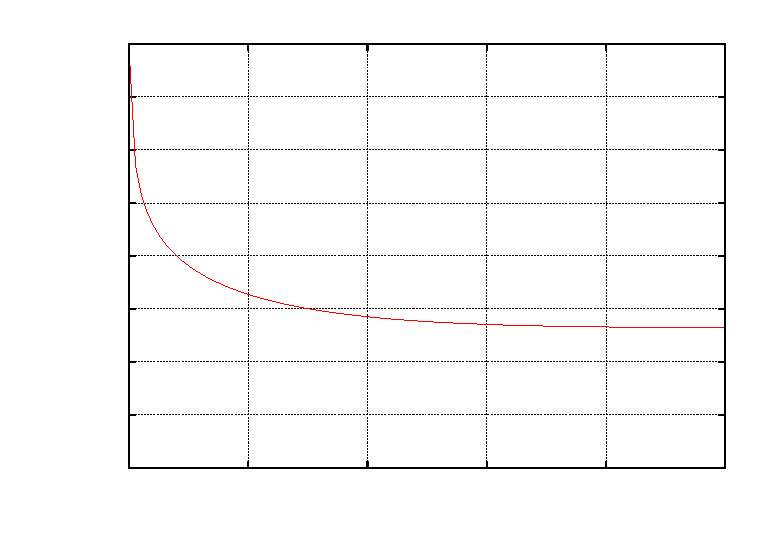
\includegraphics{sabrsmile1}}%
    \gplfronttext
  \end{picture}%
\endgroup

\end{minipage}}
\end{frame}

\begin{frame}[fragile]
\frametitle{A full example: Model diagnostics}
The markov model can generate information on the calibration process with
\begin{minted}[fontsize=\footnotesize, bgcolor=mintedBg]{c++}
std::cout << "Model trace : " << std::endl << mf->modelOutputs() 
          << std::endl;
\end{minted}
The output contains information on
\begin{itemize}
\item numerical model parameters
\item settings for smile preconditioning
\item yield term structure calibration results
\item volatility smile calibration results
\end{itemize}
and can help identifying calibration problems, resp. confirm a successful calibration.
\end{frame}


\begin{frame}[fragile]
\frametitle{A full example: Model diagnostics (model parameters / smile settings)}
\begin{minted}[fontsize=\footnotesize, bgcolor=mintedBg]{c++}
Markov functional model trace output 
Model settings
Grid points y        : 64
Std devs y           : 7
Lower rate bound     : 0
Upper rate bound     : 2
Gauss Hermite points : 32
Digital gap          : 1e-05
Adjustments          : Kahale SmileExp 
Smile moneyness checkpoints: 
\end{minted}
\end{frame}

\begin{frame}[fragile]
\frametitle{A full example: Model diagnostics (yield term structure fit)}
The raw output
\begin{minted}[fontsize=\tiny, bgcolor=mintedBg]{c++}
Yield termstructure fit:
expiry;tenor;atm;annuity;digitalAdj;ytsAdj;marketzerorate;modelzerorate;diff(bp)
November 13th, 2014;10Y;0.03047961644430512;8.267635590910791;1;1;0.03000000000000008;0.03008016185429107;-0.8016185429099432
November 12th, 2015;10Y;0.0304803836917478;8.023747530203391;1;1;0.02999999999999999;0.03003959599137232;-0.395959913723383
[...]
\end{minted}
is meant to be analyzed in another application like office
\resizebox{\textwidth}{!}{
\begin{minipage}{3.0\textwidth}
\begin{figure}
	\centering
		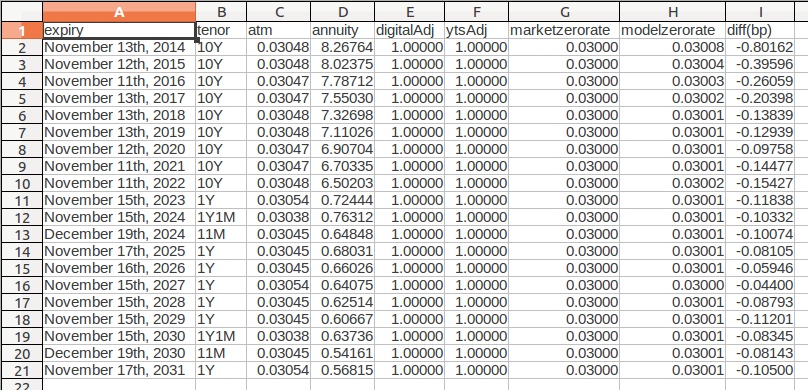
\includegraphics{office_modeltrace1.png}
\end{figure}
\end{minipage}}
\end{frame}

\begin{frame}[fragile]
\frametitle{A full example: Model diagnostics (volatility smile fit)}
\resizebox{\textwidth}{!}{
\begin{minipage}{4.0\textwidth}
\begin{figure}
	\centering
		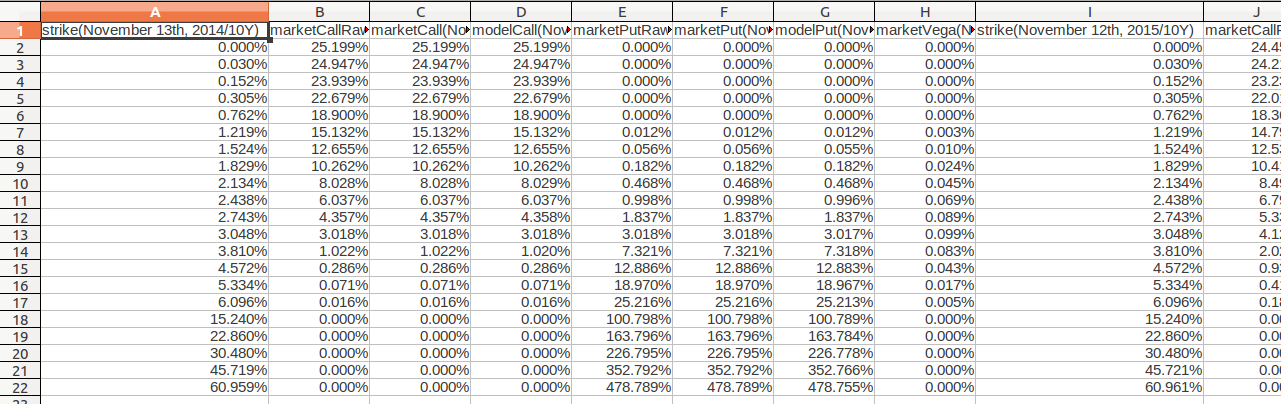
\includegraphics{office_modeltrace2.png}
\end{figure}
\end{minipage}}
\end{frame}

\section{Theoretical Background}

\frame{\frametitle{Axiomatic Hull White}
Any gaussian one factor HJM model which satisfies {\it separability}, i.e.
\begin{equation}
\sigma_f(t,T) = g(t)h(T)
\end{equation}

for the instantaneous forward rate volatility with deterministic $g, h>0$, necessarily fulfills

\begin{equation}
dr(t) = (\theta(t) - a(t)r(t)) dt + \sigma(t) dW(t) 
\end{equation}

for the short rate $r$, which means, it is a Hull White one factor model.
}

\frame{\frametitle{The T-forward numeraire}

Set $x(t) := r(t)-f(0,t)$ and fix a horizon $T$, then in the $T$-forward measure the numeraire can be written

\begin{equation}
N(t) = P(t,T) = \frac{P(0,T)}{P(0,t)} e^{-x(t)A(t,T) + B(t,T)}
\end{equation}

with $A, B$ dependent on the model parameters. The Hull White model is called an {\it affine} model.

}

\frame{\frametitle{Smile in the Hull White Model}

\begin{itemize}
\item The distribution of $N(t)$ is lognormal. The shape of the distribution can not
be controlled by any of the model parameters. 
\item For fixed $t$ you can calibrate the model to one market quoted interest rate optoin (typically a caplet or swaption).
\item You can choose the strike of the option, but the rest of the smile is implied by the model.
\end{itemize}

}

\frame{\frametitle{Callable vanilla swaps}

Pricing of callable fix versus Libor swaps may be done in a Hull White model which is calibrated as follows:

\begin{itemize}
\item For each call date find a market quoted swaption which is equivalent to the call right (in some sense, e.g. by matching the npv and its first and second
derivative of the underlying at $E(x(t))$).
\item Calibrate the volatility function $\sigma(t)$ to match the basket of these swaptions.
\item Choose the mean reversion of the model to control serial correlations.
\end{itemize}

}

\frame{\frametitle{Intertemporal correlations}

To understand the role of the reversion parameter assume $\sigma$ and $a$ constant for a moment. Then it is easy to see

\begin{equation}\label{meancorr}
\textnormal{corr}(x(T_1),x(T_2)) = \sqrt{{\frac{e^{2aT_2}-1}{e^{2aT_1}-1}}} = e^{-a(T_2-T_1)} \sqrt{ \frac{1-e^{-2aT_1}}{1-e^{-2aT_2}} }
\end{equation}

which shows that for $a=0$ the correlation is $\sqrt{T_1/T_2}$ and goes to zero if $a\rightarrow\infty$ and to one if $a\rightarrow -\infty$.

}

\frame{\frametitle{Callable cms swaps}

The calll rights in a callable cms swap are options on a swap exchanging cms coupons against fix or Libor rates. Such underlying
swaps are drastically mispriced in the Hull White model in general.

\begin{itemize}
\item cms coupons are replicated using swaptions covering the whole strike continuum $(0,\infty)$
\item The swaption smile in the Hull White model is generally not consistent with the market smile and so are the prices of cms coupons
\end{itemize}

Obviously we need a more flexible model to price such structures

}

\frame{\frametitle{Model requirements}

The wishlist for the model is as follows

\begin{itemize}
\item We want to be capable of calibrating to a whole smile of (constant maturity) swaptions, not only to one strike, for all fixing dates of the cms coupons. This is to match the coupons of the underlying. 
\item In addition we would like to calibrate to (possibly strike / maturity adjusted) coterminal swaptions to match the options representing the call rights.
\item Finally we need some control over intertemporal correlations, i.e. something operating like the reversion parameter in the Hull White model
\end{itemize}

The idea to do so is to relax the functional dependency between the state variable $x$ and the numeraire $N(t,x)$.
}

\section{Model description}

\frame{\frametitle{The driving process}

We start with a markov process driving the dynamics of the model as follows:

\begin{equation}
dx = \sigma(t) e^{at} dW(t)
\end{equation}

and $x(0) = 0$. The intertemporal correlation of the state variable $x$ is the same as for the Hull White model, see (\ref{meancorr}), i.e. the
parameter $a$ can be used to control the correlation just as the reversion parameter in the Hull White model.

}


\frame{\frametitle{The numeraire surface}

The model is operated in the $T$-forward measure, $T$ chosen big enough to cover all cashflows relevant for the actual pricing under consideration. The
link between the state $x(t)$ and the numeraire $P(t,T)$ is given by

\begin{equation}
P(t,T,x) = N(t,x)
\end{equation}

which we allow to be a non parametric surface to have maximum flexibility in calibration.
}


\section{Calibration}

\frame{\frametitle{Calibrating the numeriare surface to market smiles}

The price of a digital swaption paying out an annuity $A(t)$ on expiry $t$ if the swap rate $S(t)\geq K$ in our model is

\begin{equation}\label{modelDigital}
\textnormal{dig}_{\textnormal{model}} = P(0,T) \int_{y^*}^{\infty} \frac{A(t,y)}{P(t,T)} \phi(y) dy
\end{equation} 

where $y^*$ is the strike in the normalized state variable space (the correspondence between $y$ and $S(t)$ is constructed to be monotonic).

}

\frame{\frametitle{Implying the swap rate}

Given the market smile of $S(t)$ we can compute the market price $\textnormal{dig}_\textnormal{mkt}$(K) of digitals for strikes $K$. For given $y^*$
we can solve the equation

\begin{equation}
\textnormal{dig}_\textnormal{mkt}(K) = P(0,T) \int_{y^*}^{\infty} \frac{A(t,y)}{P(t,T)} \phi(y) dy
\end{equation}

for $K$ to find the swap rate corresponding to the state variable value $y^*$. For this $\textnormal{dig}_{mkt}(\cdot)$ should be a monotonic
function whose image is equal to the possible digital prices $(0,A(0)]$. We will revisit this later.

}

\frame{\frametitle{Computing the deflated annuity}

To compute the deflated annuity

\begin{equation}
\frac{A(t)}{P(t,T)} = \sum_{k=1}^n \tau_k \frac{P(t,t_k)}{P(t,T)}
\end{equation}

we observe that

\begin{equation}\label{deflatedZerobond}
\left.\frac{P(t,u)}{P(t,T)}\right|_{y(t)}  = E\left(\frac{1}{P(u,T)} \middle| y(t) \right)
\end{equation}

i.e. we have to integrate the reciprocal of the numeraire at future times. Working backward in time we can assume that
we know the numeraire at these times (starting with $N(T) \equiv 1$).

}

\frame{\frametitle{Converting swap rate to numeraire}

Having computed the swap rate $S(t)$ we have to convert this value to a numeraire value $N(t)$. Since

\begin{equation}
S(t)A(t) + P(t,t^*) = 1
\end{equation}

we get (by division by $N(t)$)

\begin{equation}
N(t) = \frac{1}{S(t)\frac{A(t)}{N(t)} + \frac{P(t,t^*)}{N(t)}}
\end{equation}

all terms on the right hand side computable via deflated zerobonds as shown above. Note that we use a slightly modified swap rate
here, namely one without start delay.

}

\frame{\frametitle{Calibration to a second instrument set}

Up to now we have not made use of the volatility $\sigma(t)$ in the driving markov process of the model. This parameter can be used
to calibrate the model to a second instrument set, however only a single strike can be matched obviously for each expiry. A
typical set up would be
\begin{itemize}
\item calibrate the numeraire to an underlying rate smile, e.g. constant maturity swaptions for cms coupon pricing
\item calibrate $\sigma(t)$ to (standard atm or possibly adjusted) coterminal swaptions for call right calibration
\end{itemize}
Note that after changing $\sigma(t)$ the numeraire surface needs to be updated, too.
}


\frame{\frametitle{Input smile preconditioning}

To ensure a bijective mapping

\begin{equation}
\textnormal{dig}_{\textnormal{mkt}} : (0,\infty) \rightarrow (0,A(0))
\end{equation}

it is sufficient to have an arbitrage free input smile with a $C^1$ call price function. 
It is possible to allow for negative rates and generalize
the interval $(0,\infty)$ to $(-\kappa,\infty)$ with some suitable $\kappa>0$, e.g. $\kappa = 1\%$. In general
input smiles are not arbitrage free, so some preconditioning is advisable, since arbitrageable smiles will break the
numeraire calibration.

}

\frame{\frametitle{Kahale extrapolation}

\small SABR 14y/1y implied black lognormal volatilities as of 14-11-2012, input (solid) and Kahale (dashed)

\resizebox{\textwidth}{!}{
\begin{minipage}{1.2\textwidth}
%\centering
% GNUPLOT: LaTeX picture with Postscript
\begingroup
  \makeatletter
  \providecommand\color[2][]{%
    \GenericError{(gnuplot) \space\space\space\@spaces}{%
      Package color not loaded in conjunction with
      terminal option `colourtext'%
    }{See the gnuplot documentation for explanation.%
    }{Either use 'blacktext' in gnuplot or load the package
      color.sty in LaTeX.}%
    \renewcommand\color[2][]{}%
  }%
  \providecommand\includegraphics[2][]{%
    \GenericError{(gnuplot) \space\space\space\@spaces}{%
      Package graphicx or graphics not loaded%
    }{See the gnuplot documentation for explanation.%
    }{The gnuplot epslatex terminal needs graphicx.sty or graphics.sty.}%
    \renewcommand\includegraphics[2][]{}%
  }%
  \providecommand\rotatebox[2]{#2}%
  \@ifundefined{ifGPcolor}{%
    \newif\ifGPcolor
    \GPcolortrue
  }{}%
  \@ifundefined{ifGPblacktext}{%
    \newif\ifGPblacktext
    \GPblacktexttrue
  }{}%
  % define a \g@addto@macro without @ in the name:
  \let\gplgaddtomacro\g@addto@macro
  % define empty templates for all commands taking text:
  \gdef\gplbacktext{}%
  \gdef\gplfronttext{}%
  \makeatother
  \ifGPblacktext
    % no textcolor at all
    \def\colorrgb#1{}%
    \def\colorgray#1{}%
  \else
    % gray or color?
    \ifGPcolor
      \def\colorrgb#1{\color[rgb]{#1}}%
      \def\colorgray#1{\color[gray]{#1}}%
      \expandafter\def\csname LTw\endcsname{\color{white}}%
      \expandafter\def\csname LTb\endcsname{\color{black}}%
      \expandafter\def\csname LTa\endcsname{\color{black}}%
      \expandafter\def\csname LT0\endcsname{\color[rgb]{1,0,0}}%
      \expandafter\def\csname LT1\endcsname{\color[rgb]{0,1,0}}%
      \expandafter\def\csname LT2\endcsname{\color[rgb]{0,0,1}}%
      \expandafter\def\csname LT3\endcsname{\color[rgb]{1,0,1}}%
      \expandafter\def\csname LT4\endcsname{\color[rgb]{0,1,1}}%
      \expandafter\def\csname LT5\endcsname{\color[rgb]{1,1,0}}%
      \expandafter\def\csname LT6\endcsname{\color[rgb]{0,0,0}}%
      \expandafter\def\csname LT7\endcsname{\color[rgb]{1,0.3,0}}%
      \expandafter\def\csname LT8\endcsname{\color[rgb]{0.5,0.5,0.5}}%
    \else
      % gray
      \def\colorrgb#1{\color{black}}%
      \def\colorgray#1{\color[gray]{#1}}%
      \expandafter\def\csname LTw\endcsname{\color{white}}%
      \expandafter\def\csname LTb\endcsname{\color{black}}%
      \expandafter\def\csname LTa\endcsname{\color{black}}%
      \expandafter\def\csname LT0\endcsname{\color{black}}%
      \expandafter\def\csname LT1\endcsname{\color{black}}%
      \expandafter\def\csname LT2\endcsname{\color{black}}%
      \expandafter\def\csname LT3\endcsname{\color{black}}%
      \expandafter\def\csname LT4\endcsname{\color{black}}%
      \expandafter\def\csname LT5\endcsname{\color{black}}%
      \expandafter\def\csname LT6\endcsname{\color{black}}%
      \expandafter\def\csname LT7\endcsname{\color{black}}%
      \expandafter\def\csname LT8\endcsname{\color{black}}%
    \fi
  \fi
  \setlength{\unitlength}{0.0500bp}%
  \begin{picture}(7200.00,5040.00)%
    \gplgaddtomacro\gplbacktext{%
      \csname LTb\endcsname%
      \put(946,704){\makebox(0,0)[r]{\strut{} 0}}%
      \put(946,1156){\makebox(0,0)[r]{\strut{} 0.1}}%
      \put(946,1609){\makebox(0,0)[r]{\strut{} 0.2}}%
      \put(946,2061){\makebox(0,0)[r]{\strut{} 0.3}}%
      \put(946,2513){\makebox(0,0)[r]{\strut{} 0.4}}%
      \put(946,2966){\makebox(0,0)[r]{\strut{} 0.5}}%
      \put(946,3418){\makebox(0,0)[r]{\strut{} 0.6}}%
      \put(946,3870){\makebox(0,0)[r]{\strut{} 0.7}}%
      \put(946,4323){\makebox(0,0)[r]{\strut{} 0.8}}%
      \put(946,4775){\makebox(0,0)[r]{\strut{} 0.9}}%
      \put(1078,484){\makebox(0,0){\strut{} 0}}%
      \put(2509,484){\makebox(0,0){\strut{} 0.05}}%
      \put(3941,484){\makebox(0,0){\strut{} 0.1}}%
      \put(5372,484){\makebox(0,0){\strut{} 0.15}}%
      \put(6803,484){\makebox(0,0){\strut{} 0.2}}%
      \put(176,2739){\rotatebox{-270}{\makebox(0,0){\strut{}black lognormal volatility}}}%
      \put(3940,154){\makebox(0,0){\strut{}strike}}%
    }%
    \gplgaddtomacro\gplfronttext{%
    }%
    \gplbacktext
    \put(0,0){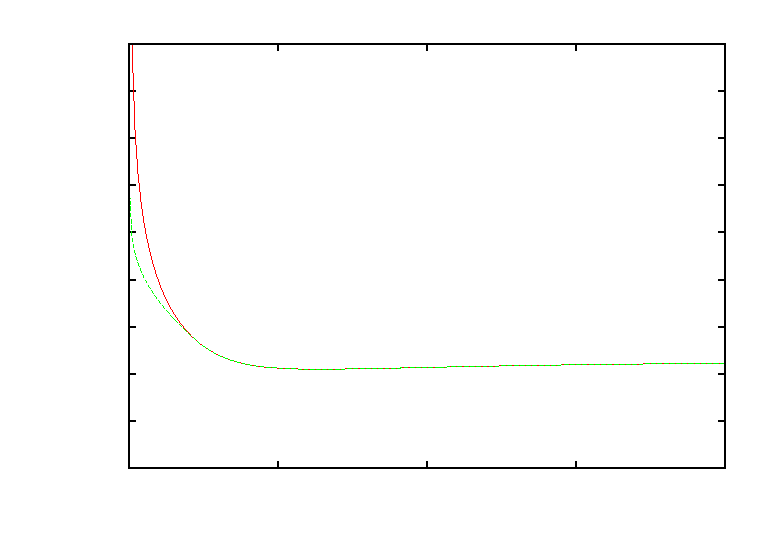
\includegraphics{MF-gnuplottex-fig2}}%
    \gplfronttext
  \end{picture}%
\endgroup

\end{minipage}}

}

\frame{\frametitle{Kahale extrapolation}

\small SABR 14y/1y call prices as of 14-11-2012, input (solid) and Kahale (dashed)

\resizebox{\textwidth}{!}{
\begin{minipage}{1.2\textwidth}
%\centering
% GNUPLOT: LaTeX picture with Postscript
\begingroup
  \makeatletter
  \providecommand\color[2][]{%
    \GenericError{(gnuplot) \space\space\space\@spaces}{%
      Package color not loaded in conjunction with
      terminal option `colourtext'%
    }{See the gnuplot documentation for explanation.%
    }{Either use 'blacktext' in gnuplot or load the package
      color.sty in LaTeX.}%
    \renewcommand\color[2][]{}%
  }%
  \providecommand\includegraphics[2][]{%
    \GenericError{(gnuplot) \space\space\space\@spaces}{%
      Package graphicx or graphics not loaded%
    }{See the gnuplot documentation for explanation.%
    }{The gnuplot epslatex terminal needs graphicx.sty or graphics.sty.}%
    \renewcommand\includegraphics[2][]{}%
  }%
  \providecommand\rotatebox[2]{#2}%
  \@ifundefined{ifGPcolor}{%
    \newif\ifGPcolor
    \GPcolortrue
  }{}%
  \@ifundefined{ifGPblacktext}{%
    \newif\ifGPblacktext
    \GPblacktexttrue
  }{}%
  % define a \g@addto@macro without @ in the name:
  \let\gplgaddtomacro\g@addto@macro
  % define empty templates for all commands taking text:
  \gdef\gplbacktext{}%
  \gdef\gplfronttext{}%
  \makeatother
  \ifGPblacktext
    % no textcolor at all
    \def\colorrgb#1{}%
    \def\colorgray#1{}%
  \else
    % gray or color?
    \ifGPcolor
      \def\colorrgb#1{\color[rgb]{#1}}%
      \def\colorgray#1{\color[gray]{#1}}%
      \expandafter\def\csname LTw\endcsname{\color{white}}%
      \expandafter\def\csname LTb\endcsname{\color{black}}%
      \expandafter\def\csname LTa\endcsname{\color{black}}%
      \expandafter\def\csname LT0\endcsname{\color[rgb]{1,0,0}}%
      \expandafter\def\csname LT1\endcsname{\color[rgb]{0,1,0}}%
      \expandafter\def\csname LT2\endcsname{\color[rgb]{0,0,1}}%
      \expandafter\def\csname LT3\endcsname{\color[rgb]{1,0,1}}%
      \expandafter\def\csname LT4\endcsname{\color[rgb]{0,1,1}}%
      \expandafter\def\csname LT5\endcsname{\color[rgb]{1,1,0}}%
      \expandafter\def\csname LT6\endcsname{\color[rgb]{0,0,0}}%
      \expandafter\def\csname LT7\endcsname{\color[rgb]{1,0.3,0}}%
      \expandafter\def\csname LT8\endcsname{\color[rgb]{0.5,0.5,0.5}}%
    \else
      % gray
      \def\colorrgb#1{\color{black}}%
      \def\colorgray#1{\color[gray]{#1}}%
      \expandafter\def\csname LTw\endcsname{\color{white}}%
      \expandafter\def\csname LTb\endcsname{\color{black}}%
      \expandafter\def\csname LTa\endcsname{\color{black}}%
      \expandafter\def\csname LT0\endcsname{\color{black}}%
      \expandafter\def\csname LT1\endcsname{\color{black}}%
      \expandafter\def\csname LT2\endcsname{\color{black}}%
      \expandafter\def\csname LT3\endcsname{\color{black}}%
      \expandafter\def\csname LT4\endcsname{\color{black}}%
      \expandafter\def\csname LT5\endcsname{\color{black}}%
      \expandafter\def\csname LT6\endcsname{\color{black}}%
      \expandafter\def\csname LT7\endcsname{\color{black}}%
      \expandafter\def\csname LT8\endcsname{\color{black}}%
    \fi
  \fi
  \setlength{\unitlength}{0.0500bp}%
  \begin{picture}(7200.00,5040.00)%
    \gplgaddtomacro\gplbacktext{%
      \csname LTb\endcsname%
      \put(1210,704){\makebox(0,0)[r]{\strut{} 0}}%
      \put(1210,1286){\makebox(0,0)[r]{\strut{} 0.005}}%
      \put(1210,1867){\makebox(0,0)[r]{\strut{} 0.01}}%
      \put(1210,2449){\makebox(0,0)[r]{\strut{} 0.015}}%
      \put(1210,3030){\makebox(0,0)[r]{\strut{} 0.02}}%
      \put(1210,3612){\makebox(0,0)[r]{\strut{} 0.025}}%
      \put(1210,4193){\makebox(0,0)[r]{\strut{} 0.03}}%
      \put(1210,4775){\makebox(0,0)[r]{\strut{} 0.035}}%
      \put(1342,484){\makebox(0,0){\strut{} 0}}%
      \put(2707,484){\makebox(0,0){\strut{} 0.05}}%
      \put(4073,484){\makebox(0,0){\strut{} 0.1}}%
      \put(5438,484){\makebox(0,0){\strut{} 0.15}}%
      \put(6803,484){\makebox(0,0){\strut{} 0.2}}%
      \put(176,2739){\rotatebox{-270}{\makebox(0,0){\strut{}call}}}%
      \put(4072,154){\makebox(0,0){\strut{}strike}}%
    }%
    \gplgaddtomacro\gplfronttext{%
    }%
    \gplbacktext
    \put(0,0){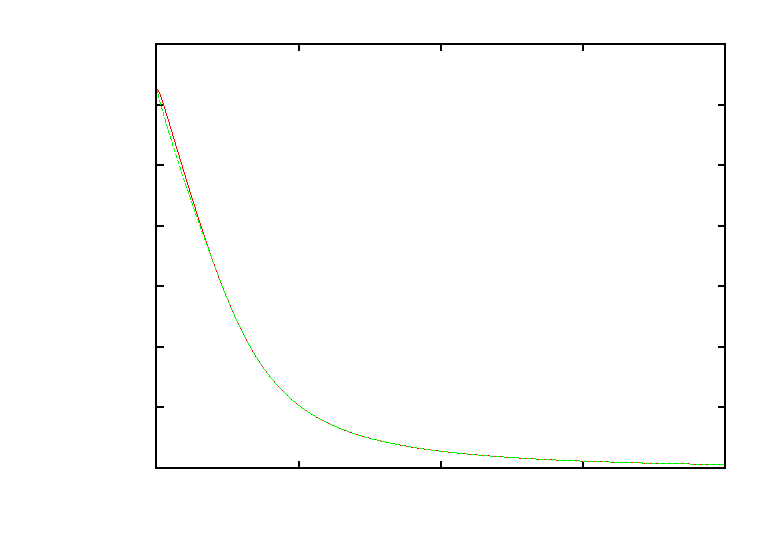
\includegraphics{MF-gnuplottex-fig3}}%
    \gplfronttext
  \end{picture}%
\endgroup

\end{minipage}}

}

\frame{\frametitle{Kahale extrapolation}

\small SABR 14y/1y digital prices as of 14-11-2012, input (solid) and Kahale (dashed)

\resizebox{\textwidth}{!}{
\begin{minipage}{1.2\textwidth}
%\centering
% GNUPLOT: LaTeX picture with Postscript
\begingroup
  \makeatletter
  \providecommand\color[2][]{%
    \GenericError{(gnuplot) \space\space\space\@spaces}{%
      Package color not loaded in conjunction with
      terminal option `colourtext'%
    }{See the gnuplot documentation for explanation.%
    }{Either use 'blacktext' in gnuplot or load the package
      color.sty in LaTeX.}%
    \renewcommand\color[2][]{}%
  }%
  \providecommand\includegraphics[2][]{%
    \GenericError{(gnuplot) \space\space\space\@spaces}{%
      Package graphicx or graphics not loaded%
    }{See the gnuplot documentation for explanation.%
    }{The gnuplot epslatex terminal needs graphicx.sty or graphics.sty.}%
    \renewcommand\includegraphics[2][]{}%
  }%
  \providecommand\rotatebox[2]{#2}%
  \@ifundefined{ifGPcolor}{%
    \newif\ifGPcolor
    \GPcolortrue
  }{}%
  \@ifundefined{ifGPblacktext}{%
    \newif\ifGPblacktext
    \GPblacktexttrue
  }{}%
  % define a \g@addto@macro without @ in the name:
  \let\gplgaddtomacro\g@addto@macro
  % define empty templates for all commands taking text:
  \gdef\gplbacktext{}%
  \gdef\gplfronttext{}%
  \makeatother
  \ifGPblacktext
    % no textcolor at all
    \def\colorrgb#1{}%
    \def\colorgray#1{}%
  \else
    % gray or color?
    \ifGPcolor
      \def\colorrgb#1{\color[rgb]{#1}}%
      \def\colorgray#1{\color[gray]{#1}}%
      \expandafter\def\csname LTw\endcsname{\color{white}}%
      \expandafter\def\csname LTb\endcsname{\color{black}}%
      \expandafter\def\csname LTa\endcsname{\color{black}}%
      \expandafter\def\csname LT0\endcsname{\color[rgb]{1,0,0}}%
      \expandafter\def\csname LT1\endcsname{\color[rgb]{0,1,0}}%
      \expandafter\def\csname LT2\endcsname{\color[rgb]{0,0,1}}%
      \expandafter\def\csname LT3\endcsname{\color[rgb]{1,0,1}}%
      \expandafter\def\csname LT4\endcsname{\color[rgb]{0,1,1}}%
      \expandafter\def\csname LT5\endcsname{\color[rgb]{1,1,0}}%
      \expandafter\def\csname LT6\endcsname{\color[rgb]{0,0,0}}%
      \expandafter\def\csname LT7\endcsname{\color[rgb]{1,0.3,0}}%
      \expandafter\def\csname LT8\endcsname{\color[rgb]{0.5,0.5,0.5}}%
    \else
      % gray
      \def\colorrgb#1{\color{black}}%
      \def\colorgray#1{\color[gray]{#1}}%
      \expandafter\def\csname LTw\endcsname{\color{white}}%
      \expandafter\def\csname LTb\endcsname{\color{black}}%
      \expandafter\def\csname LTa\endcsname{\color{black}}%
      \expandafter\def\csname LT0\endcsname{\color{black}}%
      \expandafter\def\csname LT1\endcsname{\color{black}}%
      \expandafter\def\csname LT2\endcsname{\color{black}}%
      \expandafter\def\csname LT3\endcsname{\color{black}}%
      \expandafter\def\csname LT4\endcsname{\color{black}}%
      \expandafter\def\csname LT5\endcsname{\color{black}}%
      \expandafter\def\csname LT6\endcsname{\color{black}}%
      \expandafter\def\csname LT7\endcsname{\color{black}}%
      \expandafter\def\csname LT8\endcsname{\color{black}}%
    \fi
  \fi
  \setlength{\unitlength}{0.0500bp}%
  %\begin{picture}(7200.00,5040.00)%
  \begin{picture}(6200.00,5040.00)%
    \gplgaddtomacro\gplbacktext{%
      \csname LTb\endcsname%
      \put(946,704){\makebox(0,0)[r]{\strut{} 0}}%
      \put(946,1518){\makebox(0,0)[r]{\strut{} 0.2}}%
      \put(946,2332){\makebox(0,0)[r]{\strut{} 0.4}}%
      \put(946,3147){\makebox(0,0)[r]{\strut{} 0.6}}%
      \put(946,3961){\makebox(0,0)[r]{\strut{} 0.8}}%
      \put(946,4775){\makebox(0,0)[r]{\strut{} 1}}%
      \put(1078,484){\makebox(0,0){\strut{} 0}}%
      \put(2509,484){\makebox(0,0){\strut{} 0.05}}%
      \put(3941,484){\makebox(0,0){\strut{} 0.1}}%
      \put(5372,484){\makebox(0,0){\strut{} 0.15}}%
      \put(6803,484){\makebox(0,0){\strut{} 0.2}}%
      \put(176,2739){\rotatebox{-270}{\makebox(0,0){\strut{}digital call}}}%
      \put(3940,154){\makebox(0,0){\strut{}strike}}%
    }%
    \gplgaddtomacro\gplfronttext{%
    }%
    \gplbacktext
    \put(0,0){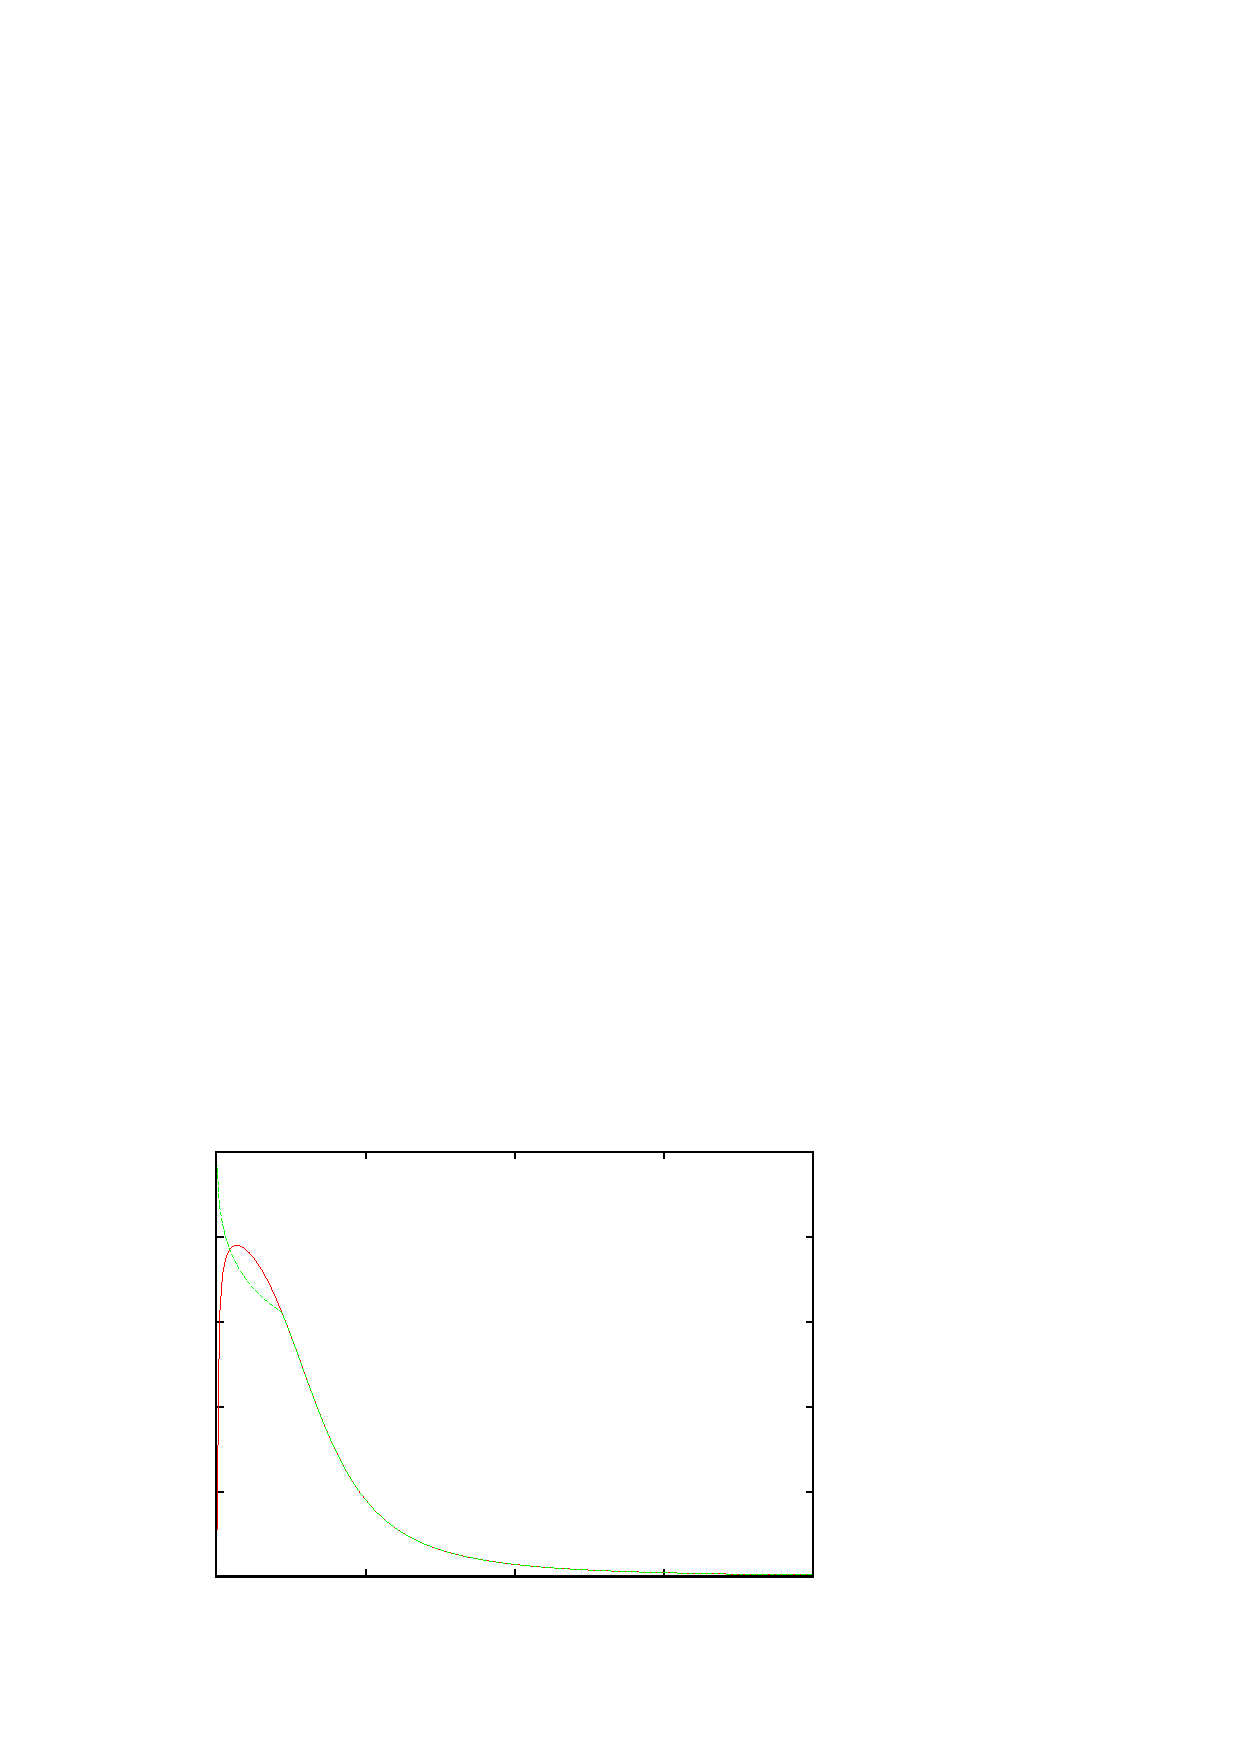
\includegraphics{MF-gnuplottex-fig4}}%
    \gplfronttext
  \end{picture}%
\endgroup

\end{minipage}}

}

\frame{\frametitle{Kahale extrapolation}

\small SABR 14y/1y density as of 14-11-2012, input (solid) and Kahale (dashed)

\resizebox{\textwidth}{!}{
\begin{minipage}{1.2\textwidth}
%\centering
% GNUPLOT: LaTeX picture with Postscript
\begingroup
  \makeatletter
  \providecommand\color[2][]{%
    \GenericError{(gnuplot) \space\space\space\@spaces}{%
      Package color not loaded in conjunction with
      terminal option `colourtext'%
    }{See the gnuplot documentation for explanation.%
    }{Either use 'blacktext' in gnuplot or load the package
      color.sty in LaTeX.}%
    \renewcommand\color[2][]{}%
  }%
  \providecommand\includegraphics[2][]{%
    \GenericError{(gnuplot) \space\space\space\@spaces}{%
      Package graphicx or graphics not loaded%
    }{See the gnuplot documentation for explanation.%
    }{The gnuplot epslatex terminal needs graphicx.sty or graphics.sty.}%
    \renewcommand\includegraphics[2][]{}%
  }%
  \providecommand\rotatebox[2]{#2}%
  \@ifundefined{ifGPcolor}{%
    \newif\ifGPcolor
    \GPcolortrue
  }{}%
  \@ifundefined{ifGPblacktext}{%
    \newif\ifGPblacktext
    \GPblacktexttrue
  }{}%
  % define a \g@addto@macro without @ in the name:
  \let\gplgaddtomacro\g@addto@macro
  % define empty templates for all commands taking text:
  \gdef\gplbacktext{}%
  \gdef\gplfronttext{}%
  \makeatother
  \ifGPblacktext
    % no textcolor at all
    \def\colorrgb#1{}%
    \def\colorgray#1{}%
  \else
    % gray or color?
    \ifGPcolor
      \def\colorrgb#1{\color[rgb]{#1}}%
      \def\colorgray#1{\color[gray]{#1}}%
      \expandafter\def\csname LTw\endcsname{\color{white}}%
      \expandafter\def\csname LTb\endcsname{\color{black}}%
      \expandafter\def\csname LTa\endcsname{\color{black}}%
      \expandafter\def\csname LT0\endcsname{\color[rgb]{1,0,0}}%
      \expandafter\def\csname LT1\endcsname{\color[rgb]{0,1,0}}%
      \expandafter\def\csname LT2\endcsname{\color[rgb]{0,0,1}}%
      \expandafter\def\csname LT3\endcsname{\color[rgb]{1,0,1}}%
      \expandafter\def\csname LT4\endcsname{\color[rgb]{0,1,1}}%
      \expandafter\def\csname LT5\endcsname{\color[rgb]{1,1,0}}%
      \expandafter\def\csname LT6\endcsname{\color[rgb]{0,0,0}}%
      \expandafter\def\csname LT7\endcsname{\color[rgb]{1,0.3,0}}%
      \expandafter\def\csname LT8\endcsname{\color[rgb]{0.5,0.5,0.5}}%
    \else
      % gray
      \def\colorrgb#1{\color{black}}%
      \def\colorgray#1{\color[gray]{#1}}%
      \expandafter\def\csname LTw\endcsname{\color{white}}%
      \expandafter\def\csname LTb\endcsname{\color{black}}%
      \expandafter\def\csname LTa\endcsname{\color{black}}%
      \expandafter\def\csname LT0\endcsname{\color{black}}%
      \expandafter\def\csname LT1\endcsname{\color{black}}%
      \expandafter\def\csname LT2\endcsname{\color{black}}%
      \expandafter\def\csname LT3\endcsname{\color{black}}%
      \expandafter\def\csname LT4\endcsname{\color{black}}%
      \expandafter\def\csname LT5\endcsname{\color{black}}%
      \expandafter\def\csname LT6\endcsname{\color{black}}%
      \expandafter\def\csname LT7\endcsname{\color{black}}%
      \expandafter\def\csname LT8\endcsname{\color{black}}%
    \fi
  \fi
  \setlength{\unitlength}{0.0500bp}%
  \begin{picture}(7200.00,5040.00)%
    \gplgaddtomacro\gplbacktext{%
      \csname LTb\endcsname%
      \put(814,1111){\makebox(0,0)[r]{\strut{}-40}}%
      \put(814,1925){\makebox(0,0)[r]{\strut{}-20}}%
      \put(814,2740){\makebox(0,0)[r]{\strut{} 0}}%
      \put(814,3554){\makebox(0,0)[r]{\strut{} 20}}%
      \put(814,4368){\makebox(0,0)[r]{\strut{} 40}}%
      \put(946,484){\makebox(0,0){\strut{} 0}}%
      \put(2410,484){\makebox(0,0){\strut{} 0.05}}%
      \put(3875,484){\makebox(0,0){\strut{} 0.1}}%
      \put(5339,484){\makebox(0,0){\strut{} 0.15}}%
      \put(6803,484){\makebox(0,0){\strut{} 0.2}}%
      \put(176,2739){\rotatebox{-270}{\makebox(0,0){\strut{}density}}}%
      \put(3874,154){\makebox(0,0){\strut{}strike}}%
    }%
    \gplgaddtomacro\gplfronttext{%
    }%
    \gplbacktext
    \put(0,0){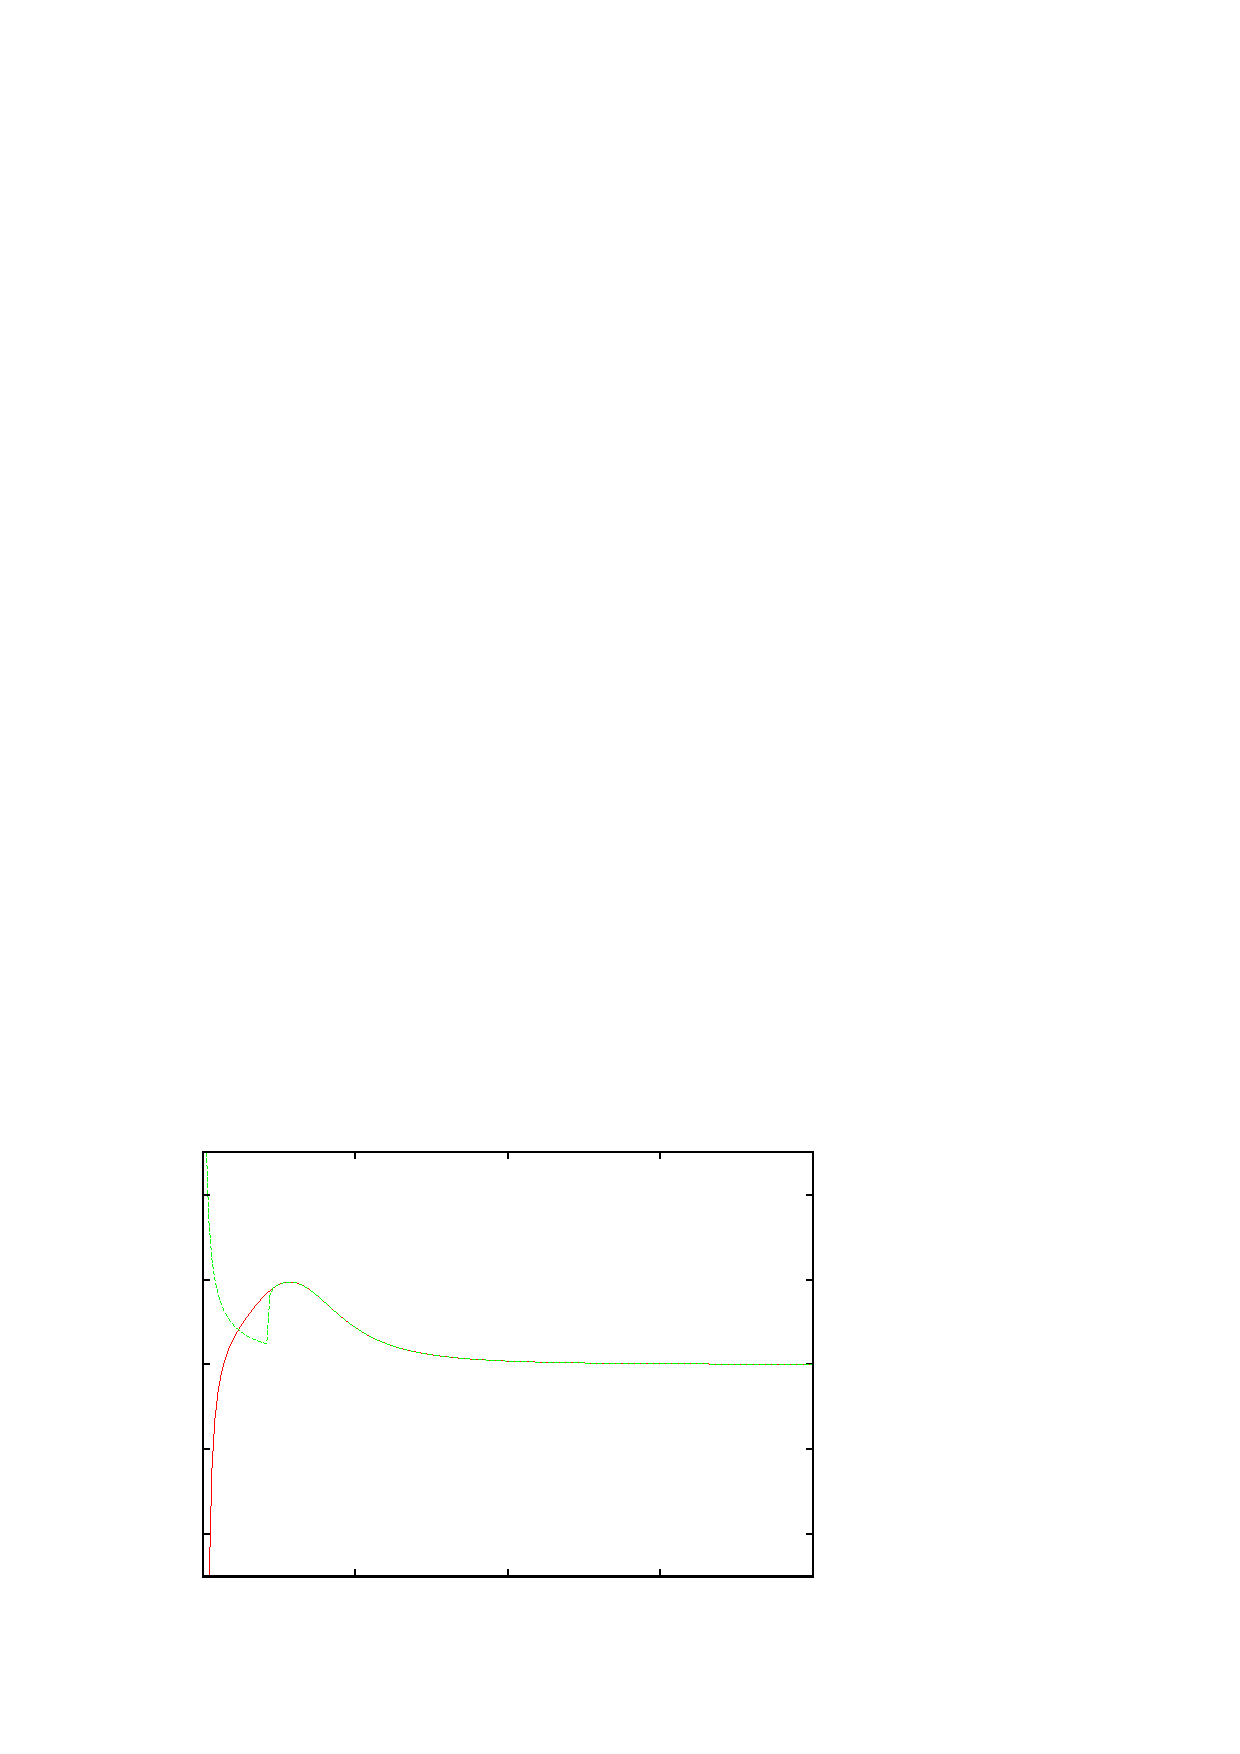
\includegraphics{MF-gnuplottex-fig5}}%
    \gplfronttext
  \end{picture}%
\endgroup

\end{minipage}}

}


\section{Numerics}

\frame{\frametitle{Interpolation of the numeraire}

In a numerical implementation of the model we will need to discretize the numeraire surface on a grid
$(t_i, y_j)$.
\begin{itemize}
\item in $y$-direction we interpolate $N(t,y)$ (normalized by todays market forward numeraire) with monotonic cubic splines
with Lagrange end condition. Outside a range of specified standard deviations (defaulted to $7$), we extrapolate flat.
\item in $t$-direction we interpolate the reciprocal of the normalized numeraire linearly. This ensures a perfect match of todays
input yield curve even for interpolated times as can easily be seen from (\ref{deflatedZerobond}). After the horizon $T$ we
extrapolate flat ($N\equiv 1$ there anyway), only for technical reasons.
\end{itemize}

}

\frame{\frametitle{Sample numeraire surface}

\small Numeraire surface for market data as of 14-11-2012

\resizebox{\textwidth}{!}{
\begin{minipage}{1.2\textwidth}
%\centering
% GNUPLOT: LaTeX picture with Postscript
\begingroup
  \makeatletter
  \providecommand\color[2][]{%
    \GenericError{(gnuplot) \space\space\space\@spaces}{%
      Package color not loaded in conjunction with
      terminal option `colourtext'%
    }{See the gnuplot documentation for explanation.%
    }{Either use 'blacktext' in gnuplot or load the package
      color.sty in LaTeX.}%
    \renewcommand\color[2][]{}%
  }%
  \providecommand\includegraphics[2][]{%
    \GenericError{(gnuplot) \space\space\space\@spaces}{%
      Package graphicx or graphics not loaded%
    }{See the gnuplot documentation for explanation.%
    }{The gnuplot epslatex terminal needs graphicx.sty or graphics.sty.}%
    \renewcommand\includegraphics[2][]{}%
  }%
  \providecommand\rotatebox[2]{#2}%
  \@ifundefined{ifGPcolor}{%
    \newif\ifGPcolor
    \GPcolortrue
  }{}%
  \@ifundefined{ifGPblacktext}{%
    \newif\ifGPblacktext
    \GPblacktexttrue
  }{}%
  % define a \g@addto@macro without @ in the name:
  \let\gplgaddtomacro\g@addto@macro
  % define empty templates for all commands taking text:
  \gdef\gplbacktext{}%
  \gdef\gplfronttext{}%
  \makeatother
  \ifGPblacktext
    % no textcolor at all
    \def\colorrgb#1{}%
    \def\colorgray#1{}%
  \else
    % gray or color?
    \ifGPcolor
      \def\colorrgb#1{\color[rgb]{#1}}%
      \def\colorgray#1{\color[gray]{#1}}%
      \expandafter\def\csname LTw\endcsname{\color{white}}%
      \expandafter\def\csname LTb\endcsname{\color{black}}%
      \expandafter\def\csname LTa\endcsname{\color{black}}%
      \expandafter\def\csname LT0\endcsname{\color[rgb]{1,0,0}}%
      \expandafter\def\csname LT1\endcsname{\color[rgb]{0,1,0}}%
      \expandafter\def\csname LT2\endcsname{\color[rgb]{0,0,1}}%
      \expandafter\def\csname LT3\endcsname{\color[rgb]{1,0,1}}%
      \expandafter\def\csname LT4\endcsname{\color[rgb]{0,1,1}}%
      \expandafter\def\csname LT5\endcsname{\color[rgb]{1,1,0}}%
      \expandafter\def\csname LT6\endcsname{\color[rgb]{0,0,0}}%
      \expandafter\def\csname LT7\endcsname{\color[rgb]{1,0.3,0}}%
      \expandafter\def\csname LT8\endcsname{\color[rgb]{0.5,0.5,0.5}}%
    \else
      % gray
      \def\colorrgb#1{\color{black}}%
      \def\colorgray#1{\color[gray]{#1}}%
      \expandafter\def\csname LTw\endcsname{\color{white}}%
      \expandafter\def\csname LTb\endcsname{\color{black}}%
      \expandafter\def\csname LTa\endcsname{\color{black}}%
      \expandafter\def\csname LT0\endcsname{\color{black}}%
      \expandafter\def\csname LT1\endcsname{\color{black}}%
      \expandafter\def\csname LT2\endcsname{\color{black}}%
      \expandafter\def\csname LT3\endcsname{\color{black}}%
      \expandafter\def\csname LT4\endcsname{\color{black}}%
      \expandafter\def\csname LT5\endcsname{\color{black}}%
      \expandafter\def\csname LT6\endcsname{\color{black}}%
      \expandafter\def\csname LT7\endcsname{\color{black}}%
      \expandafter\def\csname LT8\endcsname{\color{black}}%
    \fi
  \fi
  \setlength{\unitlength}{0.0500bp}%
  \begin{picture}(7200.00,5040.00)%
    \gplgaddtomacro\gplbacktext{%
      \csname LTb\endcsname%
      \put(6226,1259){\makebox(0,0){\strut{} 0}}%
      \put(5786,1187){\makebox(0,0){\strut{} 2}}%
      \put(5345,1115){\makebox(0,0){\strut{} 4}}%
      \put(4905,1043){\makebox(0,0){\strut{} 6}}%
      \put(4465,971){\makebox(0,0){\strut{} 8}}%
      \put(4025,899){\makebox(0,0){\strut{} 10}}%
      \put(3585,827){\makebox(0,0){\strut{} 12}}%
      \put(3145,754){\makebox(0,0){\strut{} 14}}%
      \put(955,1798){\makebox(0,0){\strut{}-3}}%
      \put(1248,1628){\makebox(0,0){\strut{}-2}}%
      \put(1540,1459){\makebox(0,0){\strut{}-1}}%
      \put(1833,1289){\makebox(0,0){\strut{} 0}}%
      \put(2125,1120){\makebox(0,0){\strut{} 1}}%
      \put(2418,950){\makebox(0,0){\strut{} 2}}%
      \put(2711,781){\makebox(0,0){\strut{} 3}}%
      \put(945,2522){\makebox(0,0)[r]{\strut{} 0}}%
      \put(945,2796){\makebox(0,0)[r]{\strut{} 0.2}}%
      \put(945,3070){\makebox(0,0)[r]{\strut{} 0.4}}%
      \put(945,3344){\makebox(0,0)[r]{\strut{} 0.6}}%
      \put(945,3619){\makebox(0,0)[r]{\strut{} 0.8}}%
      \put(945,3893){\makebox(0,0)[r]{\strut{} 1}}%
      \put(246,3299){\makebox(0,0){\strut{}N(t,y)}}%
    }%
    \gplgaddtomacro\gplfronttext{%
      \csname LTb\endcsname%
      \put(4916,829){\makebox(0,0){\strut{}t}}%
      \put(1124,1186){\makebox(0,0){\strut{}y}}%
      \put(246,3299){\makebox(0,0){\strut{}N(t,y)}}%
      \put(6641,2280){\makebox(0,0)[l]{\strut{} 0.3}}%
      \put(6641,2471){\makebox(0,0)[l]{\strut{} 0.4}}%
      \put(6641,2662){\makebox(0,0)[l]{\strut{} 0.5}}%
      \put(6641,2853){\makebox(0,0)[l]{\strut{} 0.6}}%
      \put(6641,3044){\makebox(0,0)[l]{\strut{} 0.7}}%
      \put(6641,3236){\makebox(0,0)[l]{\strut{} 0.8}}%
      \put(6641,3427){\makebox(0,0)[l]{\strut{} 0.9}}%
      \put(6641,3618){\makebox(0,0)[l]{\strut{} 1}}%
      \put(6641,3809){\makebox(0,0)[l]{\strut{} 1.1}}%
    }%
    \gplbacktext
    \put(0,0){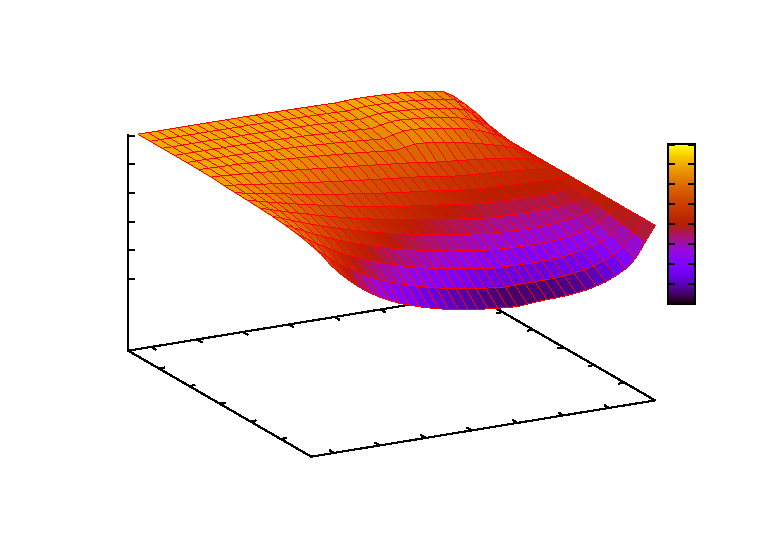
\includegraphics{MF-gnuplottex-fig1}}%
    \gplfronttext
  \end{picture}%
\endgroup

\end{minipage}}

}


\frame{\frametitle{Interpolation of payoffs}

Payoffs occuring in the numeraire bootstrap (digitals) or later in pricing exotics are also interpolated with Lagrange splines. We
leave it as an option to 
\begin{itemize}
\item restrict to integration of the payoff to a specified number of standard deviations, 
\item extrapolate the payoff flat
\item extrapolate the payoff according to the Lagrange end condition
\end{itemize}
The results should not depend significantly on this choice, otherwise the numerical parameters should be increased.

}

\frame{\frametitle{Numerical Integration for deflated zero bonds}

To compute deflated zerobond prices according to (\ref{deflatedZerobond}) it turns out that it is fast and accurate to
\begin{itemize}
\item use the celebrated Gauss Hermite Integration scheme where
\item $32$ points are more than enough usually to ensure a good accuracy.
\end{itemize}
This is because the integrand is globally well approximated by polynomials.
}

\frame{\frametitle{Numerical Integration for payoffs}

For the numerical integration of
\begin{itemize}
\item digitals during numeraire bootstrapping or 
\item exotic pricing 
\end{itemize}
Gauss Hermite is possible but not leading to satisfactory accuracy. This is due to the non global nature of the integrand in this case. Here we rely on  exact integration of the piecewise $3$rd order polynomials against the gaussian density, which is possible in closed form only involving the error function erf

}

\frame{\frametitle{How is the yield curve matched after all ?}

It is interesting to note that the initial yield curve is matched by calibrating the numeraire to market input smiles. The yield
curve is never a direct input though, as it is e.g. for the Hull White model. It is reconstructed by the model via the numeraire
density coded in and read off the market smile during numeraire bootstrapping.

}

\frame{\frametitle{Long term constant maturity calibration}

The hardest case of calibration is a long term calibration to constant maturity swaptions (or caplets).

\begin{itemize}
\item We start at maturity $T$ and bootstrap the numeraire at some $t_k < T$, introducing some numerical
noise in $N(t_k)$.
\item We then boostrap $N(t_{k-1})$ for $t_{k-1} < t_k$, relying on the already bootstrapped future numeraire
values.
\item In case of a coterminal calibration we largely still use $N(T)$ and $N(t_k)$ only to a smaller degree.
\item In case of cm calibration however we have to rely on $N(t_k)$ with $t_k$ nearer to our calibration time $t$.
\end{itemize}
Therefore in long term cm calibration numerical noise may pile up giving large errors for the shorter term numeraire
surface.

}

\frame{\frametitle{Yield curve match with standard numerical parameters}

\tiny Fit to Yts flat @ 3\%, 2y cm swaptions @ 20\%, 7 standard deviations, 200 \% upper rate bound \small
\resizebox{\textwidth}{!}{
\begin{minipage}{1.2\textwidth}
%\centering
% GNUPLOT: LaTeX picture with Postscript
\begingroup
  \makeatletter
  \providecommand\color[2][]{%
    \GenericError{(gnuplot) \space\space\space\@spaces}{%
      Package color not loaded in conjunction with
      terminal option `colourtext'%
    }{See the gnuplot documentation for explanation.%
    }{Either use 'blacktext' in gnuplot or load the package
      color.sty in LaTeX.}%
    \renewcommand\color[2][]{}%
  }%
  \providecommand\includegraphics[2][]{%
    \GenericError{(gnuplot) \space\space\space\@spaces}{%
      Package graphicx or graphics not loaded%
    }{See the gnuplot documentation for explanation.%
    }{The gnuplot epslatex terminal needs graphicx.sty or graphics.sty.}%
    \renewcommand\includegraphics[2][]{}%
  }%
  \providecommand\rotatebox[2]{#2}%
  \@ifundefined{ifGPcolor}{%
    \newif\ifGPcolor
    \GPcolortrue
  }{}%
  \@ifundefined{ifGPblacktext}{%
    \newif\ifGPblacktext
    \GPblacktexttrue
  }{}%
  % define a \g@addto@macro without @ in the name:
  \let\gplgaddtomacro\g@addto@macro
  % define empty templates for all commands taking text:
  \gdef\gplbacktext{}%
  \gdef\gplfronttext{}%
  \makeatother
  \ifGPblacktext
    % no textcolor at all
    \def\colorrgb#1{}%
    \def\colorgray#1{}%
  \else
    % gray or color?
    \ifGPcolor
      \def\colorrgb#1{\color[rgb]{#1}}%
      \def\colorgray#1{\color[gray]{#1}}%
      \expandafter\def\csname LTw\endcsname{\color{white}}%
      \expandafter\def\csname LTb\endcsname{\color{black}}%
      \expandafter\def\csname LTa\endcsname{\color{black}}%
      \expandafter\def\csname LT0\endcsname{\color[rgb]{1,0,0}}%
      \expandafter\def\csname LT1\endcsname{\color[rgb]{0,1,0}}%
      \expandafter\def\csname LT2\endcsname{\color[rgb]{0,0,1}}%
      \expandafter\def\csname LT3\endcsname{\color[rgb]{1,0,1}}%
      \expandafter\def\csname LT4\endcsname{\color[rgb]{0,1,1}}%
      \expandafter\def\csname LT5\endcsname{\color[rgb]{1,1,0}}%
      \expandafter\def\csname LT6\endcsname{\color[rgb]{0,0,0}}%
      \expandafter\def\csname LT7\endcsname{\color[rgb]{1,0.3,0}}%
      \expandafter\def\csname LT8\endcsname{\color[rgb]{0.5,0.5,0.5}}%
    \else
      % gray
      \def\colorrgb#1{\color{black}}%
      \def\colorgray#1{\color[gray]{#1}}%
      \expandafter\def\csname LTw\endcsname{\color{white}}%
      \expandafter\def\csname LTb\endcsname{\color{black}}%
      \expandafter\def\csname LTa\endcsname{\color{black}}%
      \expandafter\def\csname LT0\endcsname{\color{black}}%
      \expandafter\def\csname LT1\endcsname{\color{black}}%
      \expandafter\def\csname LT2\endcsname{\color{black}}%
      \expandafter\def\csname LT3\endcsname{\color{black}}%
      \expandafter\def\csname LT4\endcsname{\color{black}}%
      \expandafter\def\csname LT5\endcsname{\color{black}}%
      \expandafter\def\csname LT6\endcsname{\color{black}}%
      \expandafter\def\csname LT7\endcsname{\color{black}}%
      \expandafter\def\csname LT8\endcsname{\color{black}}%
    \fi
  \fi
  \setlength{\unitlength}{0.0500bp}%
  \begin{picture}(7200.00,5040.00)%
    \gplgaddtomacro\gplbacktext{%
      \csname LTb\endcsname%
      \put(1342,704){\makebox(0,0)[r]{\strut{} 0.029}}%
      \put(1342,1111){\makebox(0,0)[r]{\strut{} 0.0292}}%
      \put(1342,1518){\makebox(0,0)[r]{\strut{} 0.0294}}%
      \put(1342,1925){\makebox(0,0)[r]{\strut{} 0.0296}}%
      \put(1342,2332){\makebox(0,0)[r]{\strut{} 0.0298}}%
      \put(1342,2739){\makebox(0,0)[r]{\strut{} 0.03}}%
      \put(1342,3147){\makebox(0,0)[r]{\strut{} 0.0302}}%
      \put(1342,3554){\makebox(0,0)[r]{\strut{} 0.0304}}%
      \put(1342,3961){\makebox(0,0)[r]{\strut{} 0.0306}}%
      \put(1342,4368){\makebox(0,0)[r]{\strut{} 0.0308}}%
      \put(1342,4775){\makebox(0,0)[r]{\strut{} 0.031}}%
      \put(1474,484){\makebox(0,0){\strut{} 0}}%
      \put(2499,484){\makebox(0,0){\strut{} 10}}%
      \put(3524,484){\makebox(0,0){\strut{} 20}}%
      \put(4548,484){\makebox(0,0){\strut{} 30}}%
      \put(5573,484){\makebox(0,0){\strut{} 40}}%
      \put(6598,484){\makebox(0,0){\strut{} 50}}%
      \put(176,2739){\rotatebox{-270}{\makebox(0,0){\strut{}zero rate}}}%
      \put(4138,154){\makebox(0,0){\strut{}maturity}}%
    }%
    \gplgaddtomacro\gplfronttext{%
    }%
    \gplbacktext
    \put(0,0){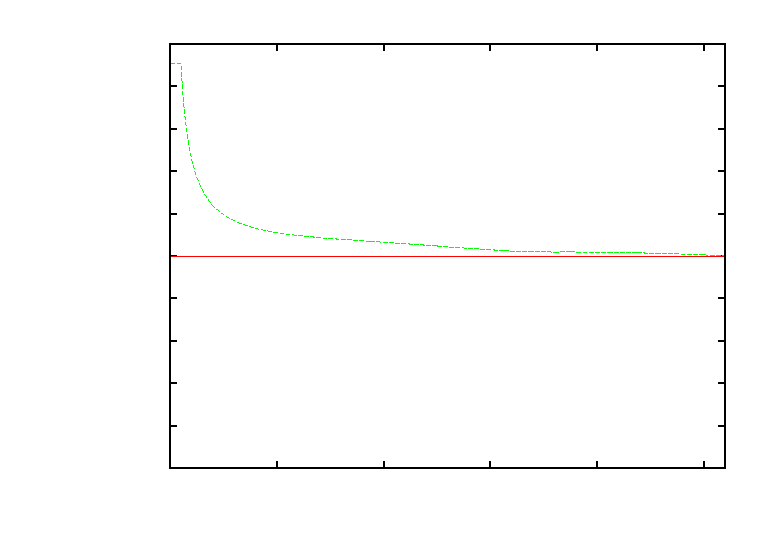
\includegraphics{MF-gnuplottex-fig6}}%
    \gplfronttext
  \end{picture}%
\endgroup

\end{minipage}}

}

\frame{\frametitle{Increasing numerical accuracy for long term cm baskets}

The first idea in this case is to increase the numerical accuracy by increasing
\begin{itemize}
\item the number of covered standard deviations (e.g. from 7 to 12)
\item the upper cut off point for rates (e.g. from 200\% to 400\%)
\item (maybe the number of discretization points, though less critical)
\end{itemize}
However this breaks the calibration totally, because the standard ("double") 53 bit mantissa numerical precision is not sufficient to do the computations numerically stable any more.
}


\begin{frame}[fragile]
\frametitle{NTL high precision computing}
The NTL and boost libraries provide support for arbitrary floating point precision. We incorporated NTL support as an option replacing
the standard double precision by an arbitrary mantissa length precision in the critical sections of the computation (which turned out to be the
integration of payoffs against the gaussian density, where large integrand values are multiplied by small density values). NTL is activated by commenting out
\begin{minted}[fontsize=\footnotesize]{c++}
// uncomment to enable NTL support
#define GAUSS1D_ENABLE_NTL 
\end{minted}
in \verb+gaussian1dmodel.hpp+. The mantissa length is then set (e.g. to 113bit) with
\begin{minted}[fontsize=\footnotesize]{c++}
boost::math::ntl::RR:SetPrecision(113)
\end{minted}
\end{frame}

\frame{\frametitle{Yield curve match using high precision computing}

\tiny Fit to Yts flat @ 3\%, 2y cm swaptions @ 20\%, 150bit mantissa, 12 standard deviations, 400 \% upper rate bound \small

\resizebox{\textwidth}{!}{
\begin{minipage}{1.2\textwidth}
%\centering
% GNUPLOT: LaTeX picture with Postscript
\begingroup
  \makeatletter
  \providecommand\color[2][]{%
    \GenericError{(gnuplot) \space\space\space\@spaces}{%
      Package color not loaded in conjunction with
      terminal option `colourtext'%
    }{See the gnuplot documentation for explanation.%
    }{Either use 'blacktext' in gnuplot or load the package
      color.sty in LaTeX.}%
    \renewcommand\color[2][]{}%
  }%
  \providecommand\includegraphics[2][]{%
    \GenericError{(gnuplot) \space\space\space\@spaces}{%
      Package graphicx or graphics not loaded%
    }{See the gnuplot documentation for explanation.%
    }{The gnuplot epslatex terminal needs graphicx.sty or graphics.sty.}%
    \renewcommand\includegraphics[2][]{}%
  }%
  \providecommand\rotatebox[2]{#2}%
  \@ifundefined{ifGPcolor}{%
    \newif\ifGPcolor
    \GPcolortrue
  }{}%
  \@ifundefined{ifGPblacktext}{%
    \newif\ifGPblacktext
    \GPblacktexttrue
  }{}%
  % define a \g@addto@macro without @ in the name:
  \let\gplgaddtomacro\g@addto@macro
  % define empty templates for all commands taking text:
  \gdef\gplbacktext{}%
  \gdef\gplfronttext{}%
  \makeatother
  \ifGPblacktext
    % no textcolor at all
    \def\colorrgb#1{}%
    \def\colorgray#1{}%
  \else
    % gray or color?
    \ifGPcolor
      \def\colorrgb#1{\color[rgb]{#1}}%
      \def\colorgray#1{\color[gray]{#1}}%
      \expandafter\def\csname LTw\endcsname{\color{white}}%
      \expandafter\def\csname LTb\endcsname{\color{black}}%
      \expandafter\def\csname LTa\endcsname{\color{black}}%
      \expandafter\def\csname LT0\endcsname{\color[rgb]{1,0,0}}%
      \expandafter\def\csname LT1\endcsname{\color[rgb]{0,1,0}}%
      \expandafter\def\csname LT2\endcsname{\color[rgb]{0,0,1}}%
      \expandafter\def\csname LT3\endcsname{\color[rgb]{1,0,1}}%
      \expandafter\def\csname LT4\endcsname{\color[rgb]{0,1,1}}%
      \expandafter\def\csname LT5\endcsname{\color[rgb]{1,1,0}}%
      \expandafter\def\csname LT6\endcsname{\color[rgb]{0,0,0}}%
      \expandafter\def\csname LT7\endcsname{\color[rgb]{1,0.3,0}}%
      \expandafter\def\csname LT8\endcsname{\color[rgb]{0.5,0.5,0.5}}%
    \else
      % gray
      \def\colorrgb#1{\color{black}}%
      \def\colorgray#1{\color[gray]{#1}}%
      \expandafter\def\csname LTw\endcsname{\color{white}}%
      \expandafter\def\csname LTb\endcsname{\color{black}}%
      \expandafter\def\csname LTa\endcsname{\color{black}}%
      \expandafter\def\csname LT0\endcsname{\color{black}}%
      \expandafter\def\csname LT1\endcsname{\color{black}}%
      \expandafter\def\csname LT2\endcsname{\color{black}}%
      \expandafter\def\csname LT3\endcsname{\color{black}}%
      \expandafter\def\csname LT4\endcsname{\color{black}}%
      \expandafter\def\csname LT5\endcsname{\color{black}}%
      \expandafter\def\csname LT6\endcsname{\color{black}}%
      \expandafter\def\csname LT7\endcsname{\color{black}}%
      \expandafter\def\csname LT8\endcsname{\color{black}}%
    \fi
  \fi
  \setlength{\unitlength}{0.0500bp}%
  \begin{picture}(7200.00,5040.00)%
    \gplgaddtomacro\gplbacktext{%
      \csname LTb\endcsname%
      \put(1606,704){\makebox(0,0)[r]{\strut{} 0.02999}}%
      \put(1606,1111){\makebox(0,0)[r]{\strut{} 0.029992}}%
      \put(1606,1518){\makebox(0,0)[r]{\strut{} 0.029994}}%
      \put(1606,1925){\makebox(0,0)[r]{\strut{} 0.029996}}%
      \put(1606,2332){\makebox(0,0)[r]{\strut{} 0.029998}}%
      \put(1606,2739){\makebox(0,0)[r]{\strut{} 0.03}}%
      \put(1606,3147){\makebox(0,0)[r]{\strut{} 0.030002}}%
      \put(1606,3554){\makebox(0,0)[r]{\strut{} 0.030004}}%
      \put(1606,3961){\makebox(0,0)[r]{\strut{} 0.030006}}%
      \put(1606,4368){\makebox(0,0)[r]{\strut{} 0.030008}}%
      \put(1606,4775){\makebox(0,0)[r]{\strut{} 0.03001}}%
      \put(1738,484){\makebox(0,0){\strut{} 0}}%
      \put(2712,484){\makebox(0,0){\strut{} 10}}%
      \put(3686,484){\makebox(0,0){\strut{} 20}}%
      \put(4660,484){\makebox(0,0){\strut{} 30}}%
      \put(5634,484){\makebox(0,0){\strut{} 40}}%
      \put(6608,484){\makebox(0,0){\strut{} 50}}%
      \put(176,2739){\rotatebox{-270}{\makebox(0,0){\strut{}zero rate}}}%
      \put(4270,154){\makebox(0,0){\strut{}maturity}}%
    }%
    \gplgaddtomacro\gplfronttext{%
    }%
    \gplbacktext
    \put(0,0){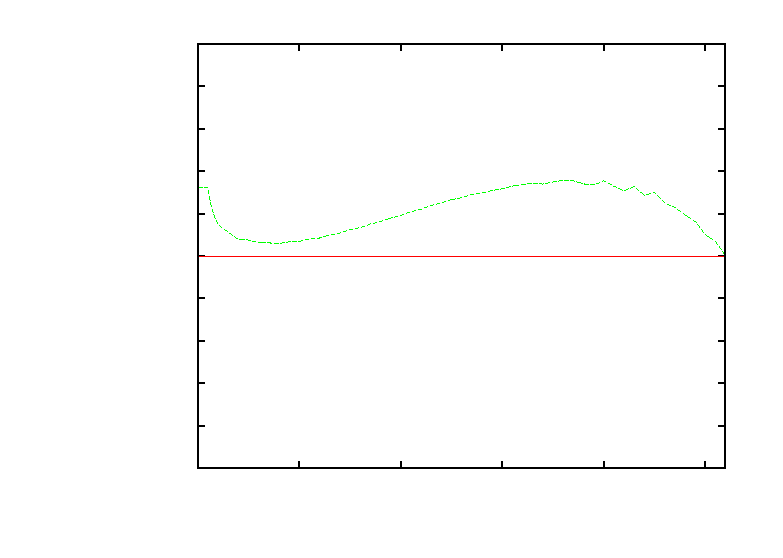
\includegraphics{MF-gnuplottex-fig7}}%
    \gplfronttext
  \end{picture}%
\endgroup

\end{minipage}}

}

\frame{\frametitle{A more pragmatic approach: Adjustment factors}

Computations with NTL are slow. A more practical way to stabilize the calibration in difficult circumstances are adjustment factors forcing
the numeraire to match the market input yield curve. The adjustment factor is introduced by replacing

\begin{equation}
N(t_i,y_j) \rightarrow N(t_i,y_j) \frac{P^{\textnormal{model}}(0,t_i)}{P^{\textnormal{market}}(0,t_i)}
\end{equation}

This option should be used with some care because it may lower the accuracy of the volatility smile match. In most situations the adjustment factors are moderate though, in the example we had before:

}

\frame{\frametitle{Adjustment factors in the example above}

\begin{table}[ht]
\begin{tabular}{l | l}
Date & Adjustment Factor \\ \hline
  November 14th, 2013 & 1.00000029079227 \\
  November 14th, 2014 & 0.999999566861981 \\
  November 14th, 2015 & 0.999999720414697 \\
  November 14th, 2016 & 0.999999838009949 \\
  November 14th, 2017 & 0.999999380770489 \\
 ... & ... \\
  November 14th, 2056 & 0.999804362556495 \\
  November 14th, 2057 & 0.999904959217797 \\
  November 14th, 2058 & 0.99988000473961 \\
  November 14th, 2059 & 0.999816723715493 \\
  November 14th, 2060 & 0.999830021528368 \\
  November 14th, 2061 & 0.999737006370401 \\
  November 14th, 2062 & 0.999761860227793 \\
  November 14th, 2063 & 0.999887598113548 \\
\end{tabular}
\label{adjfactors}
\end{table}

}

\begin{frame}[fragile]
\frametitle{MarkovFunctional Options - Numerical Parameters}
\begin{itemize}
\item \verb+yGridPoint+ Number of discretization points for normalized state variable (default $64$)
\item \verb+yStdDevs+ Number of standard deviations of normalized state variable covered (default $7$)
\item \verb+gaussHermitePoints+ Number of points used in Gauss hermite integration (default $32$)
\item \verb+digitalGap+ Numerical stepsize to compute market digitals from call spreads (default $10^{-5}$)
\item \verb+marketRateAccuracy+ Accuracy (in model swap rate) when matching market digitals (default $10^{-7}$)
\item \verb+lowerRateBound+ Lower bound for model's (underlying) rates (default $0\%$)
\item \verb+upperRateBound+ Upper bound for model's (underlying) rates (default $200\%$)
\end{itemize}
\end{frame}

\begin{frame}[fragile]
\frametitle{MarkovFunctional Options - Adjustments Overview}
\begin{itemize}
\item \verb+AdjustDigitals+ -- force the model's digital at the lower rate bound to be $1$.
Limited impact, not recommended, does not seem to be useful in practice.
\item \verb+AdjustYts+ -- force the model's yts to match the input yts by applying a constant
adjustment factor per expiry. Recommended only for very long term calibrations,
smile fit may suffer
\item \verb+ExtrapolatePayoffFlat+ -- Instead of extrapolating using the spline, extrapolate the digital's
payoff flat outside the given standard deviations of the state variable. Recommended only for sanity
checks, should have no impact, otherwise numerical parameters have to be adjusted
\item \verb+NoPayoffExtrapolation+ -- Do not extrapolate the payoff at all. Same as for ExtrapolatePayoffFlat
holds
\end{itemize}
\end{frame}


\begin{frame}[fragile]
\frametitle{MarkovFunctional Options - Adjustments Overview ctd.}
\begin{itemize}
\item \verb+KahaleSmile+ -- Use Kahale smile preconditioning on arbitrageable wings, recommended (or \verb+SabrSmile+) unless
you are sure to provide an arbitrage free smile input
\item \verb+KahaleInterpolation+ -- Use Kahale smile interpolation (implies \verb+KahaleSmile+), for naively interpolated smiles
(linear, ...), however generates ``Bat Man shaped'' Densities, not recommended unless \verb+SabrSmile+ fails to work or is too
inaccurate w.r.t. fit
\item \verb+SmileExponentialExtrapolation+ -- Use Exponential smile extrapolation on right wing (implies \verb+KahaleSmile+),
for slowly decreasing call price functions, recommended
\end{itemize}
\end{frame}

\begin{frame}[fragile]
\frametitle{MarkovFunctional Options - Adjustments Overview ctd.}
\begin{itemize}
\item \verb+SmileDeleteArbitragePoints+ -- Delete intermediate points from smile that cause arbitrage (implies \verb+KahaleInterpolation+),
recommended if you use \verb+KahaleInterpolation+
\item \verb+SabrSmile+ -- Use a Sabr fitted smile (with Kahale wing sanitization), recommended for naively interpolated smiles
\item \verb+SmileMoneynessCheckPoints+ -- Custom strike grid for smile arbitrage check and Kahale interpolation in $K/F$ space (optional),
default is working in most cases
\end{itemize}
\end{frame}

\section{Secondary instrument set calibration}

\begin{frame}[fragile]
\frametitle{Representative Basket Approach}
We are coming back to the question to which secondary instrument basket we
should calibrate to represent cms / float (or other exotic) swaptions.
\begin{itemize}
\item Problem: Find standard swaptions that represent an exotic call right
appropriately in your Markov Functional (or any one factor) model.
\item Strategy: Match NPV, Delta\footnote{which means the first derivative
w.r.t. the state variable of the model here}, Gamma around some ``central''
value of the model's state variable.
This works well for amortizing, accreting and step up/down swaptions for
example. It is worth a try if we can use the method also in our initial
example with the CMS swaption.
\end{itemize}
\end{frame}

\begin{frame}[fragile]
\frametitle{Global amortizing vanilla swap fit}
(solid = exotic npv, dotted = standard underlying npv)
\resizebox{\textwidth}{!}{
\begin{minipage}{1.2\textwidth}
\begin{figure}
	\centering
         % GNUPLOT: LaTeX picture with Postscript
\begingroup
  \makeatletter
  \providecommand\color[2][]{%
    \GenericError{(gnuplot) \space\space\space\@spaces}{%
      Package color not loaded in conjunction with
      terminal option `colourtext'%
    }{See the gnuplot documentation for explanation.%
    }{Either use 'blacktext' in gnuplot or load the package
      color.sty in LaTeX.}%
    \renewcommand\color[2][]{}%
  }%
  \providecommand\includegraphics[2][]{%
    \GenericError{(gnuplot) \space\space\space\@spaces}{%
      Package graphicx or graphics not loaded%
    }{See the gnuplot documentation for explanation.%
    }{The gnuplot epslatex terminal needs graphicx.sty or graphics.sty.}%
    \renewcommand\includegraphics[2][]{}%
  }%
  \providecommand\rotatebox[2]{#2}%
  \@ifundefined{ifGPcolor}{%
    \newif\ifGPcolor
    \GPcolortrue
  }{}%
  \@ifundefined{ifGPblacktext}{%
    \newif\ifGPblacktext
    \GPblacktexttrue
  }{}%
  % define a \g@addto@macro without @ in the name:
  \let\gplgaddtomacro\g@addto@macro
  % define empty templates for all commands taking text:
  \gdef\gplbacktext{}%
  \gdef\gplfronttext{}%
  \makeatother
  \ifGPblacktext
    % no textcolor at all
    \def\colorrgb#1{}%
    \def\colorgray#1{}%
  \else
    % gray or color?
    \ifGPcolor
      \def\colorrgb#1{\color[rgb]{#1}}%
      \def\colorgray#1{\color[gray]{#1}}%
      \expandafter\def\csname LTw\endcsname{\color{white}}%
      \expandafter\def\csname LTb\endcsname{\color{black}}%
      \expandafter\def\csname LTa\endcsname{\color{black}}%
      \expandafter\def\csname LT0\endcsname{\color[rgb]{1,0,0}}%
      \expandafter\def\csname LT1\endcsname{\color[rgb]{0,1,0}}%
      \expandafter\def\csname LT2\endcsname{\color[rgb]{0,0,1}}%
      \expandafter\def\csname LT3\endcsname{\color[rgb]{1,0,1}}%
      \expandafter\def\csname LT4\endcsname{\color[rgb]{0,1,1}}%
      \expandafter\def\csname LT5\endcsname{\color[rgb]{1,1,0}}%
      \expandafter\def\csname LT6\endcsname{\color[rgb]{0,0,0}}%
      \expandafter\def\csname LT7\endcsname{\color[rgb]{1,0.3,0}}%
      \expandafter\def\csname LT8\endcsname{\color[rgb]{0.5,0.5,0.5}}%
    \else
      % gray
      \def\colorrgb#1{\color{black}}%
      \def\colorgray#1{\color[gray]{#1}}%
      \expandafter\def\csname LTw\endcsname{\color{white}}%
      \expandafter\def\csname LTb\endcsname{\color{black}}%
      \expandafter\def\csname LTa\endcsname{\color{black}}%
      \expandafter\def\csname LT0\endcsname{\color{black}}%
      \expandafter\def\csname LT1\endcsname{\color{black}}%
      \expandafter\def\csname LT2\endcsname{\color{black}}%
      \expandafter\def\csname LT3\endcsname{\color{black}}%
      \expandafter\def\csname LT4\endcsname{\color{black}}%
      \expandafter\def\csname LT5\endcsname{\color{black}}%
      \expandafter\def\csname LT6\endcsname{\color{black}}%
      \expandafter\def\csname LT7\endcsname{\color{black}}%
      \expandafter\def\csname LT8\endcsname{\color{black}}%
    \fi
  \fi
  \setlength{\unitlength}{0.0500bp}%
  \begin{picture}(7200.00,5040.00)%
    \gplgaddtomacro\gplbacktext{%
      \csname LTb\endcsname%
      \put(814,704){\makebox(0,0)[r]{\strut{}-20}}%
      \put(814,1383){\makebox(0,0)[r]{\strut{}-15}}%
      \put(814,2061){\makebox(0,0)[r]{\strut{}-10}}%
      \put(814,2740){\makebox(0,0)[r]{\strut{}-5}}%
      \put(814,3418){\makebox(0,0)[r]{\strut{} 0}}%
      \put(814,4097){\makebox(0,0)[r]{\strut{} 5}}%
      \put(814,4775){\makebox(0,0)[r]{\strut{} 10}}%
      \put(1532,484){\makebox(0,0){\strut{}-4}}%
      \put(2703,484){\makebox(0,0){\strut{}-2}}%
      \put(3875,484){\makebox(0,0){\strut{} 0}}%
      \put(5046,484){\makebox(0,0){\strut{} 2}}%
      \put(6217,484){\makebox(0,0){\strut{} 4}}%
      \put(176,2739){\rotatebox{-270}{\makebox(0,0){\strut{}npv}}}%
      \put(3874,154){\makebox(0,0){\strut{}y}}%
    }%
    \gplgaddtomacro\gplfronttext{%
    }%
    \gplbacktext
    \put(0,0){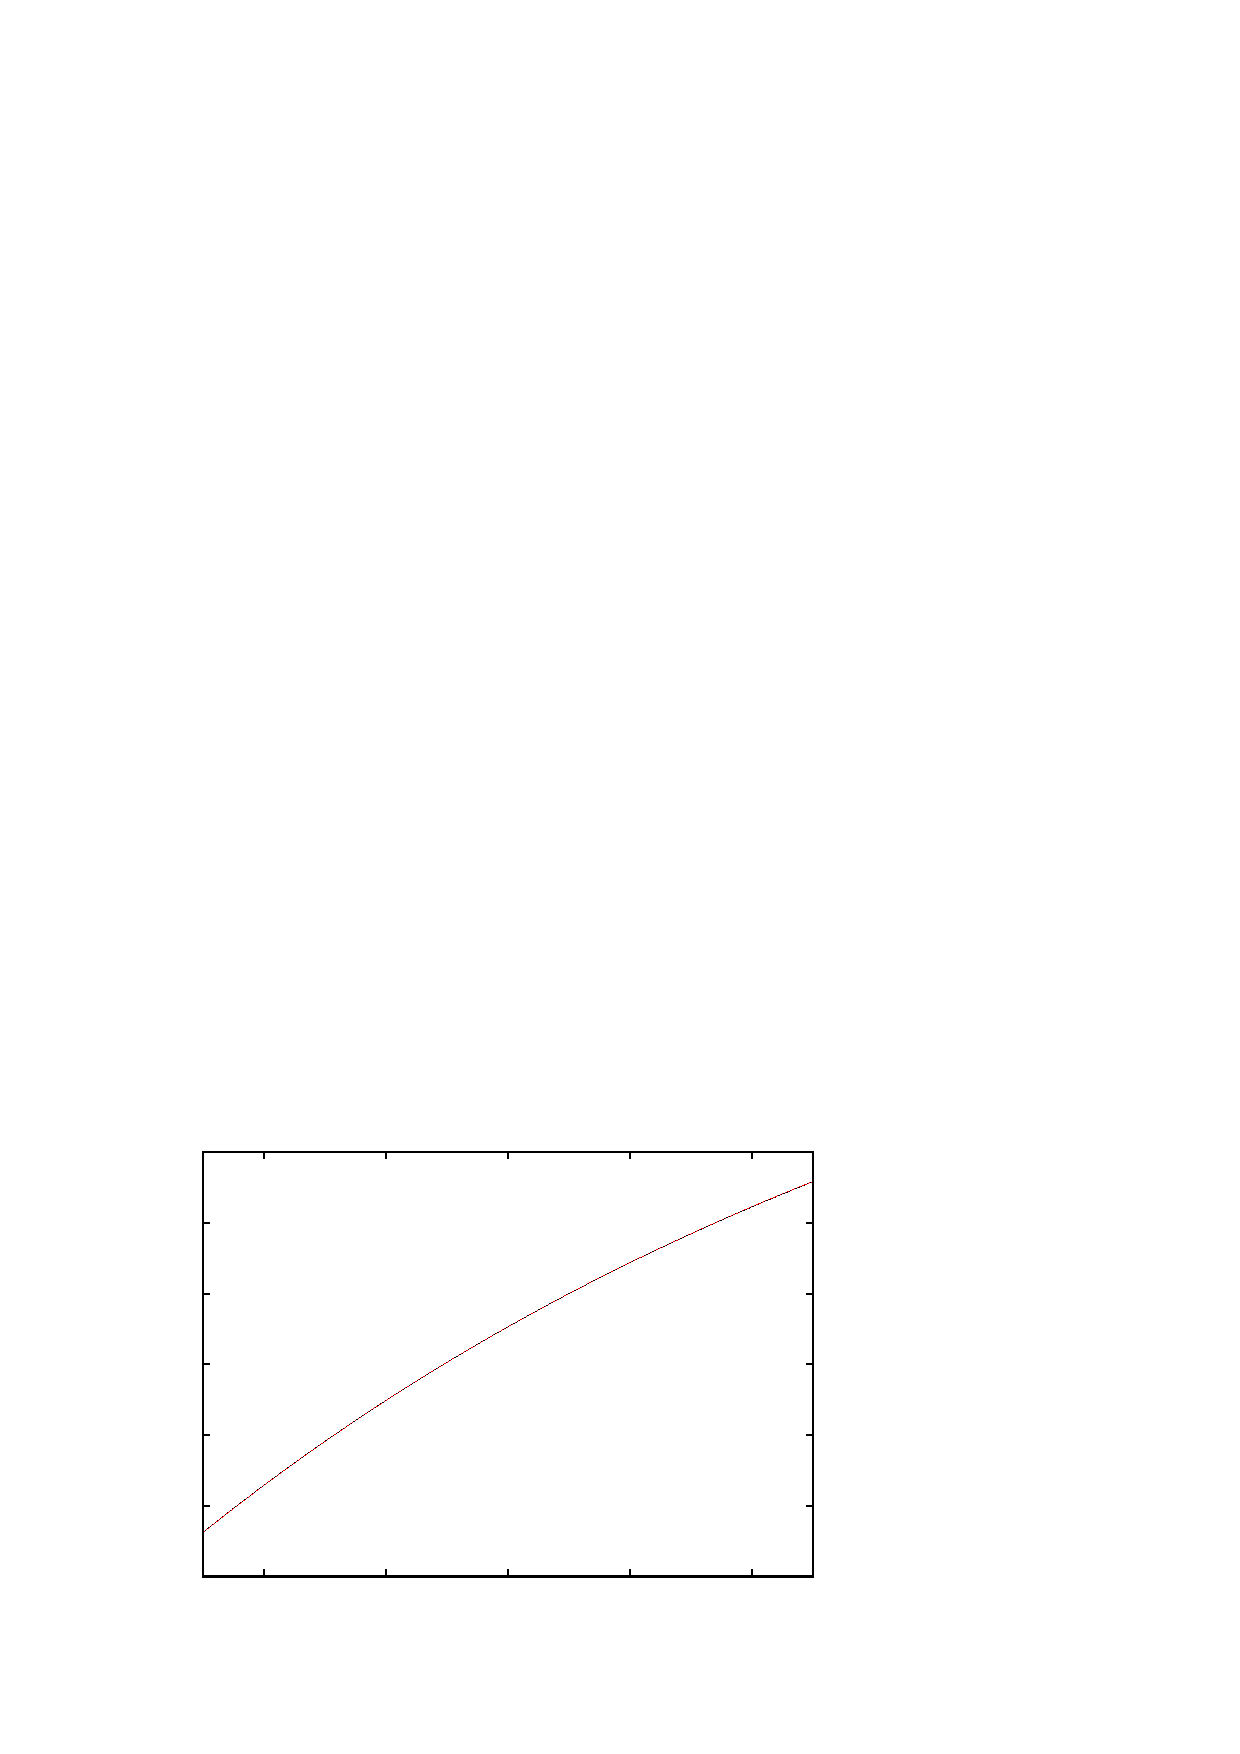
\includegraphics{representativeBasket-gnuplottex-fig1}}%
    \gplfronttext
  \end{picture}%
\endgroup

\end{figure}
\end{minipage}}
\end{frame}


\begin{frame}[fragile]
\frametitle{Global CMS swap fit (Flat smile)}
(solid = exotic npv, dotted = standard underlying npv)
\resizebox{\textwidth}{!}{
\begin{minipage}{1.2\textwidth}
\begin{figure}
	\centering
         % GNUPLOT: LaTeX picture with Postscript
\begingroup
  \makeatletter
  \providecommand\color[2][]{%
    \GenericError{(gnuplot) \space\space\space\@spaces}{%
      Package color not loaded in conjunction with
      terminal option `colourtext'%
    }{See the gnuplot documentation for explanation.%
    }{Either use 'blacktext' in gnuplot or load the package
      color.sty in LaTeX.}%
    \renewcommand\color[2][]{}%
  }%
  \providecommand\includegraphics[2][]{%
    \GenericError{(gnuplot) \space\space\space\@spaces}{%
      Package graphicx or graphics not loaded%
    }{See the gnuplot documentation for explanation.%
    }{The gnuplot epslatex terminal needs graphicx.sty or graphics.sty.}%
    \renewcommand\includegraphics[2][]{}%
  }%
  \providecommand\rotatebox[2]{#2}%
  \@ifundefined{ifGPcolor}{%
    \newif\ifGPcolor
    \GPcolortrue
  }{}%
  \@ifundefined{ifGPblacktext}{%
    \newif\ifGPblacktext
    \GPblacktexttrue
  }{}%
  % define a \g@addto@macro without @ in the name:
  \let\gplgaddtomacro\g@addto@macro
  % define empty templates for all commands taking text:
  \gdef\gplbacktext{}%
  \gdef\gplfronttext{}%
  \makeatother
  \ifGPblacktext
    % no textcolor at all
    \def\colorrgb#1{}%
    \def\colorgray#1{}%
  \else
    % gray or color?
    \ifGPcolor
      \def\colorrgb#1{\color[rgb]{#1}}%
      \def\colorgray#1{\color[gray]{#1}}%
      \expandafter\def\csname LTw\endcsname{\color{white}}%
      \expandafter\def\csname LTb\endcsname{\color{black}}%
      \expandafter\def\csname LTa\endcsname{\color{black}}%
      \expandafter\def\csname LT0\endcsname{\color[rgb]{1,0,0}}%
      \expandafter\def\csname LT1\endcsname{\color[rgb]{0,1,0}}%
      \expandafter\def\csname LT2\endcsname{\color[rgb]{0,0,1}}%
      \expandafter\def\csname LT3\endcsname{\color[rgb]{1,0,1}}%
      \expandafter\def\csname LT4\endcsname{\color[rgb]{0,1,1}}%
      \expandafter\def\csname LT5\endcsname{\color[rgb]{1,1,0}}%
      \expandafter\def\csname LT6\endcsname{\color[rgb]{0,0,0}}%
      \expandafter\def\csname LT7\endcsname{\color[rgb]{1,0.3,0}}%
      \expandafter\def\csname LT8\endcsname{\color[rgb]{0.5,0.5,0.5}}%
    \else
      % gray
      \def\colorrgb#1{\color{black}}%
      \def\colorgray#1{\color[gray]{#1}}%
      \expandafter\def\csname LTw\endcsname{\color{white}}%
      \expandafter\def\csname LTb\endcsname{\color{black}}%
      \expandafter\def\csname LTa\endcsname{\color{black}}%
      \expandafter\def\csname LT0\endcsname{\color{black}}%
      \expandafter\def\csname LT1\endcsname{\color{black}}%
      \expandafter\def\csname LT2\endcsname{\color{black}}%
      \expandafter\def\csname LT3\endcsname{\color{black}}%
      \expandafter\def\csname LT4\endcsname{\color{black}}%
      \expandafter\def\csname LT5\endcsname{\color{black}}%
      \expandafter\def\csname LT6\endcsname{\color{black}}%
      \expandafter\def\csname LT7\endcsname{\color{black}}%
      \expandafter\def\csname LT8\endcsname{\color{black}}%
    \fi
  \fi
  \setlength{\unitlength}{0.0500bp}%
  \begin{picture}(7200.00,5040.00)%
    \gplgaddtomacro\gplbacktext{%
      \csname LTb\endcsname%
      \put(1210,704){\makebox(0,0)[r]{\strut{}-25000}}%
      \put(1210,1383){\makebox(0,0)[r]{\strut{}-20000}}%
      \put(1210,2061){\makebox(0,0)[r]{\strut{}-15000}}%
      \put(1210,2740){\makebox(0,0)[r]{\strut{}-10000}}%
      \put(1210,3418){\makebox(0,0)[r]{\strut{}-5000}}%
      \put(1210,4097){\makebox(0,0)[r]{\strut{} 0}}%
      \put(1210,4775){\makebox(0,0)[r]{\strut{} 5000}}%
      \put(1888,484){\makebox(0,0){\strut{}-4}}%
      \put(2980,484){\makebox(0,0){\strut{}-2}}%
      \put(4073,484){\makebox(0,0){\strut{} 0}}%
      \put(5165,484){\makebox(0,0){\strut{} 2}}%
      \put(6257,484){\makebox(0,0){\strut{} 4}}%
      \put(176,2739){\rotatebox{-270}{\makebox(0,0){\strut{}npv}}}%
      \put(4072,154){\makebox(0,0){\strut{}y}}%
    }%
    \gplgaddtomacro\gplfronttext{%
    }%
    \gplbacktext
    \put(0,0){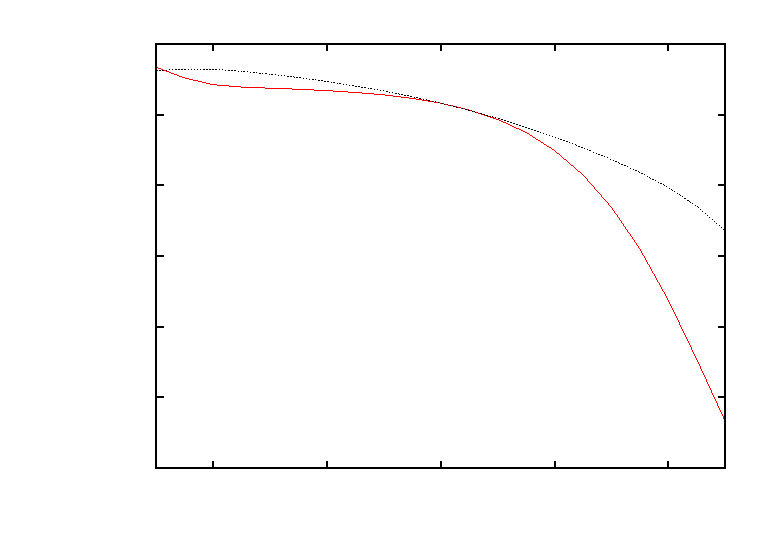
\includegraphics{representativeBasket-gnuplottex-fig3}}%
    \gplfronttext
  \end{picture}%
\endgroup

\end{figure}
\end{minipage}}
\end{frame}

\begin{frame}[fragile]
\frametitle{Global CMS swap fit (SABR smile)}
(solid = exotic npv, dotted = standard underlying npv)
\resizebox{\textwidth}{!}{
\begin{minipage}{1.2\textwidth}
\begin{figure}
	\centering
         % GNUPLOT: LaTeX picture with Postscript
\begingroup
  \makeatletter
  \providecommand\color[2][]{%
    \GenericError{(gnuplot) \space\space\space\@spaces}{%
      Package color not loaded in conjunction with
      terminal option `colourtext'%
    }{See the gnuplot documentation for explanation.%
    }{Either use 'blacktext' in gnuplot or load the package
      color.sty in LaTeX.}%
    \renewcommand\color[2][]{}%
  }%
  \providecommand\includegraphics[2][]{%
    \GenericError{(gnuplot) \space\space\space\@spaces}{%
      Package graphicx or graphics not loaded%
    }{See the gnuplot documentation for explanation.%
    }{The gnuplot epslatex terminal needs graphicx.sty or graphics.sty.}%
    \renewcommand\includegraphics[2][]{}%
  }%
  \providecommand\rotatebox[2]{#2}%
  \@ifundefined{ifGPcolor}{%
    \newif\ifGPcolor
    \GPcolortrue
  }{}%
  \@ifundefined{ifGPblacktext}{%
    \newif\ifGPblacktext
    \GPblacktexttrue
  }{}%
  % define a \g@addto@macro without @ in the name:
  \let\gplgaddtomacro\g@addto@macro
  % define empty templates for all commands taking text:
  \gdef\gplbacktext{}%
  \gdef\gplfronttext{}%
  \makeatother
  \ifGPblacktext
    % no textcolor at all
    \def\colorrgb#1{}%
    \def\colorgray#1{}%
  \else
    % gray or color?
    \ifGPcolor
      \def\colorrgb#1{\color[rgb]{#1}}%
      \def\colorgray#1{\color[gray]{#1}}%
      \expandafter\def\csname LTw\endcsname{\color{white}}%
      \expandafter\def\csname LTb\endcsname{\color{black}}%
      \expandafter\def\csname LTa\endcsname{\color{black}}%
      \expandafter\def\csname LT0\endcsname{\color[rgb]{1,0,0}}%
      \expandafter\def\csname LT1\endcsname{\color[rgb]{0,1,0}}%
      \expandafter\def\csname LT2\endcsname{\color[rgb]{0,0,1}}%
      \expandafter\def\csname LT3\endcsname{\color[rgb]{1,0,1}}%
      \expandafter\def\csname LT4\endcsname{\color[rgb]{0,1,1}}%
      \expandafter\def\csname LT5\endcsname{\color[rgb]{1,1,0}}%
      \expandafter\def\csname LT6\endcsname{\color[rgb]{0,0,0}}%
      \expandafter\def\csname LT7\endcsname{\color[rgb]{1,0.3,0}}%
      \expandafter\def\csname LT8\endcsname{\color[rgb]{0.5,0.5,0.5}}%
    \else
      % gray
      \def\colorrgb#1{\color{black}}%
      \def\colorgray#1{\color[gray]{#1}}%
      \expandafter\def\csname LTw\endcsname{\color{white}}%
      \expandafter\def\csname LTb\endcsname{\color{black}}%
      \expandafter\def\csname LTa\endcsname{\color{black}}%
      \expandafter\def\csname LT0\endcsname{\color{black}}%
      \expandafter\def\csname LT1\endcsname{\color{black}}%
      \expandafter\def\csname LT2\endcsname{\color{black}}%
      \expandafter\def\csname LT3\endcsname{\color{black}}%
      \expandafter\def\csname LT4\endcsname{\color{black}}%
      \expandafter\def\csname LT5\endcsname{\color{black}}%
      \expandafter\def\csname LT6\endcsname{\color{black}}%
      \expandafter\def\csname LT7\endcsname{\color{black}}%
      \expandafter\def\csname LT8\endcsname{\color{black}}%
    \fi
  \fi
  \setlength{\unitlength}{0.0500bp}%
  \begin{picture}(7200.00,5040.00)%
    \gplgaddtomacro\gplbacktext{%
      \csname LTb\endcsname%
      \put(1210,704){\makebox(0,0)[r]{\strut{}-25000}}%
      \put(1210,1383){\makebox(0,0)[r]{\strut{}-20000}}%
      \put(1210,2061){\makebox(0,0)[r]{\strut{}-15000}}%
      \put(1210,2740){\makebox(0,0)[r]{\strut{}-10000}}%
      \put(1210,3418){\makebox(0,0)[r]{\strut{}-5000}}%
      \put(1210,4097){\makebox(0,0)[r]{\strut{} 0}}%
      \put(1210,4775){\makebox(0,0)[r]{\strut{} 5000}}%
      \put(1888,484){\makebox(0,0){\strut{}-4}}%
      \put(2980,484){\makebox(0,0){\strut{}-2}}%
      \put(4073,484){\makebox(0,0){\strut{} 0}}%
      \put(5165,484){\makebox(0,0){\strut{} 2}}%
      \put(6257,484){\makebox(0,0){\strut{} 4}}%
      \put(176,2739){\rotatebox{-270}{\makebox(0,0){\strut{}npv}}}%
      \put(4072,154){\makebox(0,0){\strut{}y}}%
    }%
    \gplgaddtomacro\gplfronttext{%
    }%
    \gplbacktext
    \put(0,0){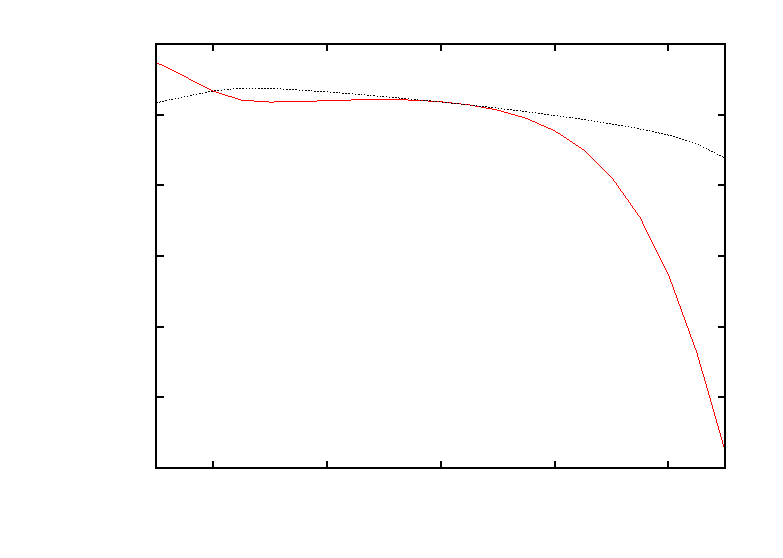
\includegraphics{representativeBasket-gnuplottex-fig4}}%
    \gplfronttext
  \end{picture}%
\endgroup

\end{figure}
\end{minipage}}
\end{frame}


\begin{frame}[fragile]
\frametitle{Representative Basket Approach - Conclusion}
It does not seem to be clear to what secondary instrument set you
should calibrate your model in order to represent calls on a cms
(or more generally float float) swaps, although in practice atm
coterminals seem to be a common choice. 
\end{frame}


\section{Implementation in QuantLib}

\frame{\frametitle{QuantLib Implementation}

A base version of the model is available since release $1.3$. Recent developemts ($\geq 1.4$ ?) include

\begin{itemize}
\item support for a (zero volatility) spread between discounting and forwarding curves 
\item a float float and non standard swaption pricing engine
\item representative calibration basket generation
\item support for pricing under credit risk (credit linked swaptions, exotic bonds)
\item SABR-Kahale smile preconditioning
\end{itemize}

}


\frame{\frametitle{Outlook / Future Tasks}

\begin{itemize}
\item Finite Difference pricing engines
\item Additional smile preconditioning algorithms
\end{itemize}

}

\section{References}

\frame{\frametitle{References}

\begin{itemize}

\item Johnson, Simon: Numerical methods for the markov functional model, Wilmott magazine, \small http://www.wilmott.com/pdfs/110802\_johnson.pdf \normalsize

\item Kahale, Nabil: An arbitrage free interpolation of volatilities, Risk May 2004, 
\small  http://nkahale.free.fr/papers/Interpolation.pdf  \normalsize

\item Shoup, Victor: NTL A Library for doing Number theory, \small http://www.shoup.net/ntl/ \normalsize

\item QuantLib A free/open-source library for quantitative finance, \small http://www.quantlib.org \normalsize

\item Caspers, Peter: Markov Functional One Factor Interest Rate Model Implementation in QuantLib, \small http://papers.ssrn.com/sol3/papers.cfm?abstract\_id=2183721 \normalsize

\item Caspers, Peter: Representative Basket Method Applied, \small http://papers.ssrn.com/sol3/papers.cfm?abstract\_id=2320759 \normalsize

\end{itemize}

}


\section{Questions}

\frame{\frametitle{Thank you,  Questions ?}
\begin{figure}
	\centering
		\includegraphics{/home/peter/Pictures/Beaker2.png}
\end{figure}

}



\end{document}

